\documentclass[a4paper]{article}

%\usepackage{fullpage}
\usepackage[margin=3.0cm]{geometry}

\usepackage[T1]{fontenc}
\usepackage[english]{babel}
\usepackage{textcomp}
\usepackage{multirow}
\usepackage{float}
\usepackage{fancyhdr}
\usepackage{pdfpages}
\usepackage{longtable}
\usepackage{fancyref}
\setcounter{secnumdepth}{5}


\usepackage{hyperref}
\hypersetup{
	pdfauthor = {Henrik Sohlberg},
	pdftitle = {eh2770: Assignment 2: JDH Insurance},
	pdfsubject = {EH2770},
	pdfkeywords = {EAAT, MAP},
	pdfcreator = {LaTeX with hyperref package},
	pdfproducer = {latex}
}

\usepackage{graphicx}
\usepackage{amsmath}


\title{Assignment II \\Architectural Change of J.D.H. Insurance}

\author{Henrik Sohlberg <\href{mailto:hsoh@kth.se}{hsoh@kth.se}> \\%
		Jonas Eyob <\href{mailto:eyob@kth.se}{eyob@kth.se}> \\%
		Daniel R\"onnow <\href{mailto:ronnow@kth.se}{ronnow@kth.se}>
}

\fancyhf{}
\fancyhead[LE,RO]{\slshape \rightmark}
\fancyhead[LO,RE]{\slshape \leftmark}
\fancyfoot[C]{\thepage}

\begin{document}
\thispagestyle{empty}
\maketitle
\thispagestyle{empty}
\pagestyle{empty}
\newpage    
\tableofcontents
\newpage
\pagestyle{fancy}
\setcounter{page}{1}

\section{Introduction}
\label{sec:introduction}
This report intends to overview the J.D.H. Insurance's, a fictive company, enterprise architecture as it is today, and subsequently describe models, suggestions for improvements and plan the transition from the as-is architecture to the to-be. The scope has been limited to the section in the organisation where the external customer plays an active role, including business processes such as when a customer orders an insurance, reports a claim, needs support, and also internal processes supporting these main processes.
\subsection{J.D.H. Insurance}
\label{sec:j_d_h_insurance}
J.D.H. Insurance is an insurance company with focus on private persons. The company has, during some years, increased their number of customers constantly, making the company one of the leading insurance companies in the country. This has lead to many changes throughout the years and the CEO and other managers has during the last years experienced that the informations systems does not support the business enough to deliver value to the business and customers along with increasing cost for the systems. The company is now in need of, and want to transform the architecture into a more efficient and standardized enterprise architecture. This they believe could be reached by analyzing their current architecture and develop it into an architecture more supporting, more standardized and more cost-efficient.
\subsection{Vision Statement}
\label{sec:vision_statement}
J.D.H. Insurance's intention is to become the greatest company providing insurance to customers in terms of products, support, and value. It shall be pleasurable to become a customer through each of the company's sale channels. It shall be satisfying to be a customer, with tremendous support and service.
\subsection{Goals}
\label{sec:goals}
The goal with this paper is to analyze the processes included in the above mentioned scope to approach the visions stated. J.D.H. Insurance can become a greater company by increasing the accuracy in the claim registration to support the decision making of such claim and to increase the availability of the support processes to ensure customer satisfaction in case of arising problems. By increasing the availability of the sales channels, the process of ordering an insurance can be more pleasurable to the customer. A reduced cost of the same process could be exploited by J.D.H. Insurance to become more competitive in compensating customers, which also creates value to them.
\subsection{EA Utilities}
\label{sec:ea_utilities}
The work of this architectural change uses two distinct utilities for executing the analyze and finding an architecture aligning with the requirements of the CEO and the other stakeholders. The first utility is the Multi Attribute Prediction metamodel (MAP, \vref{sec:map_metamodel}) which is capable of assigning values to attributes of the modeled entities to be able to analyze the models with specific attributes in mind. The second is the Enterprise Architecture Analysis Tool (EAAT, \vref{sec:eaat}) which is an application capable of modeling using the MAP metamodel and is capable of running analyzes. These utilities are further explained in the coming sections.
\subsubsection{ArchiMate}
\label{sec:archimate}
ArchiMate, a modelling language specified by The Open Group, offers a common way to model an enterprise architecture. It is based on three layers - business, application, and technology - providing the possibility to unambiguously describe, analyze, and visualize complex structures within an organization. Each layer consists of objects describing a certain element within a specific layer.
\subsubsection{MAP Metamodel}
\label{sec:map_metamodel}
The Multi Attribute Prediction model (MAP) is based on the ArchiMate language and can be described as an extension to it, enabling further analysis of an enterprise architecture . The tool uses the same concept with layers and services and adds the functionality of assigning attribute values to elements. These attributes are application modifiability, data accuracy, application usage, service availability, interoperability, cost, and utility.\\\\
%
\textbf{Application modifiability} is of great interest when analyzing IT-system architecture as the metric determines how complex it is to modify and replace existing modules and/or systems. For example, several systems may probably be interconnected, if we replace one of them - how much work will be needed to make the new structure operational? The Application modifiability attribute seeks to answer this question and in general help decision makers in similar situations. The value is based on three metrics for an application: complexity, size, and coupling.\\\\
%
\textbf{Data accuracy} refers to the quality of data in terms of correctness and error. Low data accuracy may be the result of the human factor, when it was manually inputted to a system. As data flow through the enterprise, it is important to define data accuracy to be able to analyze the impact certain data have to the whole system.\\\\
%
As the portfolio of systems within an organization grows, the likelihood of having redundant applications increases. At the same time, it can be difficult to understand the importance of a system. A tool to analyze this issue is to calculate the Application usage, which (not surprisingly) indicate the usage for an application. Roughly, the value is calculated based on how a user perceive a technology to fulfill a work task.\\\\
%
\textbf{Service availability} refers to the attribute value describing the availability for a service. This value is determined by statistics regarding the fail-ratio/down-time and time consumed on maintenance on a system. The availability attribute is often rated very highly by IT-system executive since the costs are often of serious magnitude when a system is failing.\\\\
%
\textbf{Interoperability} refers to the the communication between different systems. The attribute is used to display which systems that are interoperable. If they "speak" the same language, they can exchange information and thus are interoperable, otherwise not.\\\\
%
The attribute \textbf{Cost} is, straightforwardly, important and useful information in an enterprise architecture. In MAP, the cost consists of the initial cost and the yearly cost, which refers to maintenance and support etc.\\\\
%
The \textbf{Utility} attribute belongs to a stakeholder and it is a function dependent on a stakeholder's requirements for a service or an application. The value is useful to view the impact a system and its properties has, in terms of utility, for a stakeholder.
%
\subsubsection{EAAT tool}
\label{sec:eaat}
The Enterprise Architecture Analysis Tool (EAAT) is developed by the school of Electrical Engineering at the Royal Institute of Technology and is capable of modelling and calculating analyzes of an enterprise and the enterprise's information systems. The analysis done in EAAT can be used to support decision making in reaching the target architecture from the vision of the enterprise. The analysis focuses on attributes in the metamodel, and by using MAP as metamodel and EAAT for modelling and analyzing J.D.H. Insurance's enterprise, their vision can be reached by analyzing scenarios to find the most suitable target architecture.
%
\subsection{IT-systems}
\label{sec:it_systems}
Supporting the business processes within the enterprise are a set of IT-systems addressing a certain needs of the company. Next, the IT-systems used by J.D.H. Insurance are presented briefly.
%
\subsubsection{Customer Relationship Management}
\label{sec:crm}
Customer Relationship Management (CRM) is a system for analyzing and managing the interaction with existing and potential customers. Through the different capabilities commonly offered by these systems companies can build a more personal relations with the customer and thereby achieve a higher degree of customer satisfaction. In the context of J.D.H. Insurance the CRM system provides means of identifying potential customer needs based on observed customer behaviour.
\subsubsection{Enterprise Resource Planning}
\label{sec:erp}
In the scope of this report the Enterprise Resource Planning (ERP) is a system used for maintaining various information flows within the boundaries of the organization. In J.D.H. Insurance the ERP is used for registering the different compensation claims.      
\subsubsection{Claim Management System}
\label{sec:cms}
The Claim Management System (CMS) is a system within J.D.H. Insurance that handles all claim related inquiries; the functionality of the CMS include, but are not limited to: providing a digitized form for claim reporting, providing claim information connected to a specific customer, customer compensation payment etc. This system in turn collaborates with other systems for performing certain tasks (this is depicted in the models below).
\subsubsection{Mail Support System}
\label{sec:mss}
The Mail Support System (MSS) used in J.D.H. Insurance is a system that utilizes a help desk DB and a mail server in order to offer functionality for: handling of in- and outgoing issue mail as well as providing the help desk worker with a set of tools to ease the work of problem solving. 
\subsubsection{Order Management System}
\label{sec:oms}
The Order Management System (OMS) is the entity within the order flow responsible for handling insurance orders. It uses an independent database for order storage and also collaborates with a CRM system for retrieval of customer information as well as coupling order(s) to customer.  


\clearpage

%\section{The As-Is Architecture}
\section{As-Is}
\label{sec:as_is}
The As-Is architecture of J.D.H. Insurance is derived from their most important processes. From these processes the information systems, information objects and technical infrastructure can be identified. The following sections will present each of these important processes and their underlying systems, objects and infrastructure.
\subsection{J.D.H. Insurance's most core processes, systems and objects}
\label{sec:coreShit}
The models presented in this section considers the As-is state of the enterprise architecture. The following subsections will describe the important functions in J.D.H. Insurance and each function will be followed by a model explaining the business processes and objects, information system and the underlying technology. These models are high-level overview ArchiMate models of the processes and systems to give a picture of the enterprise and they may differ slightly from the later presented As-Is model in the MAP language.
\subsubsection{The Ordering of an Insurance}
\label{sec:order}
To order an insurance the customer is able to browse J.D.H. Insurance's website for the insurance they would like to apply for. The customer is then able to download a paper application form and send it to J.D.H. Insurance by mail for the company's order managers to register the order and to send an order status response back to the customer before the order of an insurance is completed. \Fref{fig:archi_order} shows the business services available for the customer and what processes they are realised by, which system that supports these processes and the objects used when ordering an insurance.
\begin{center}
	\begin{figure}[H]
		\centering
		\setlength\fboxsep{7pt}
		\setlength\fboxrule{0.5pt}
		\fbox{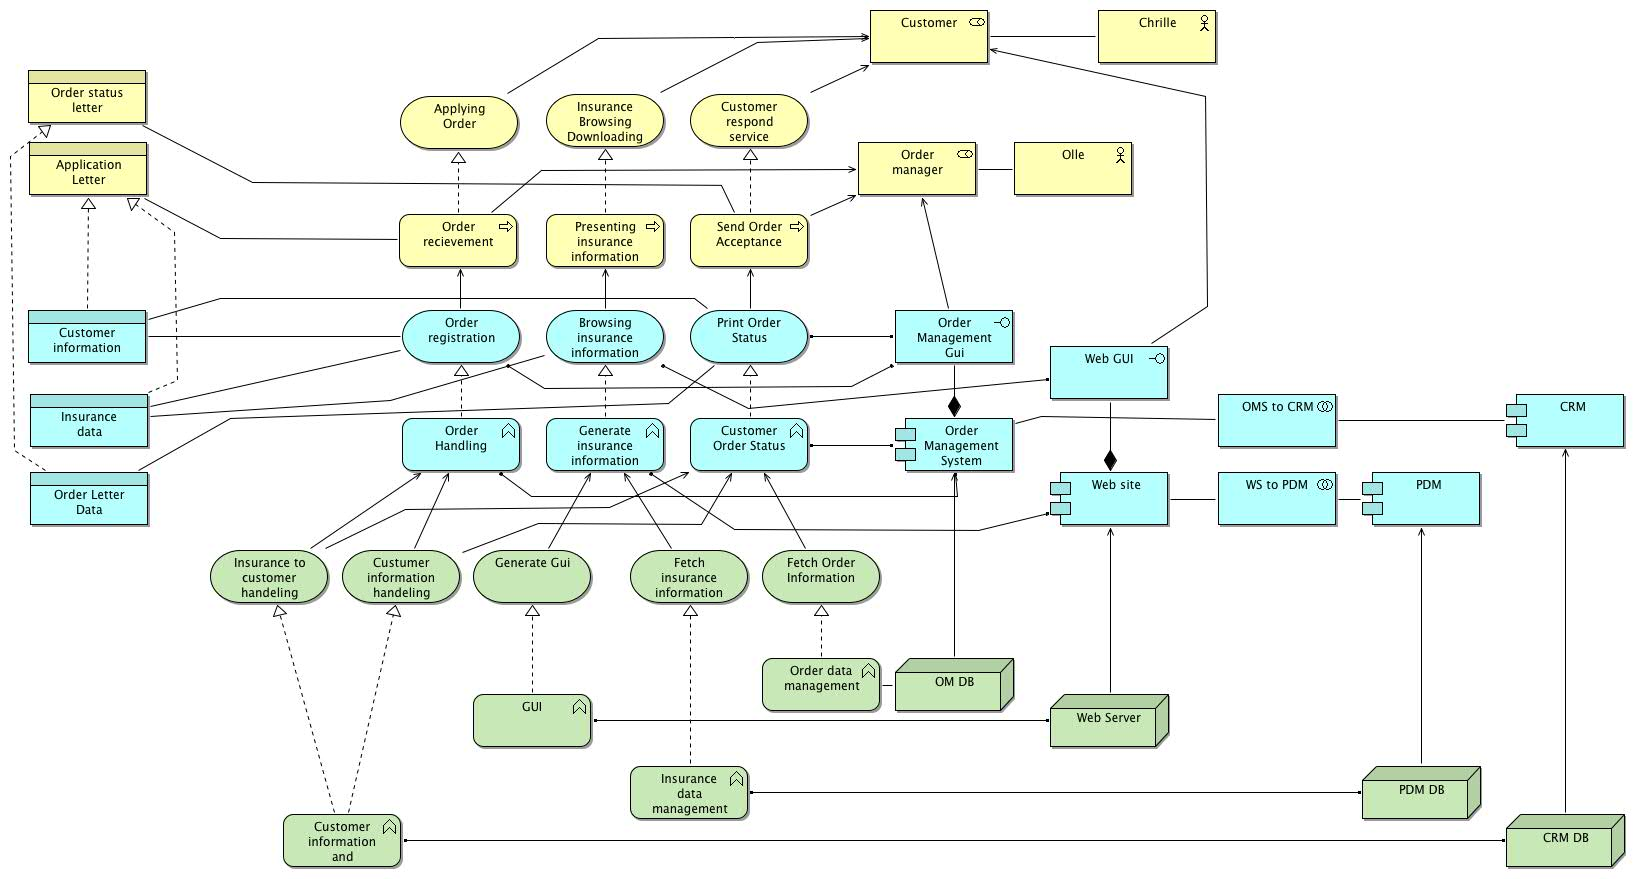
\includegraphics[scale = 0.252]{images/order.jpg}}
		\caption{Ordering an insurance (\emph{ArchiMate})}
		\label{fig:archi_order}
	\end{figure}
\end{center}
\subsubsection{The Process of Claim Registration}
\label{sec:claim}
To claim compensation, the customer are able to download a paper claim application from the website. The application, including customer information and claim description, is sent to J.D.H Insurance by mail which is received by a claim administrator which registers it in the Claim management system by hand. A Claim Evaluator evaluates the claim application and compensates the customer in case of valid claim. Either way the claim evaluator notifies the customer by sending a letter with his answer to the claim. \Fref{fig:archi_claim} displays the services available to the customer and the underlying process and systems. It also shows the processes which the evaluator and administrator executes and which systems they use.
\begin{center}
	\begin{figure}[H]
		\centering
		\setlength\fboxsep{7pt}
		\setlength\fboxrule{0.5pt}
		\fbox{\includegraphics[scale = 0.245]{images/claim.png}}
		\caption{Claim registration (\emph{ArchiMate})}
		\label{fig:archi_claim}
	\end{figure}
\end{center}
%
\subsubsection{Support Processes}
\label{sec:support_processes}
J.D.H. Insurance provides various support services for their customers and possible customers, which includes support by phone or e-mail. Each support service are described in the following subsections.
\paragraph{Phone Support}
\label{sec:phone}
The customer has the option to call in to J.D.H. Insurance for support. \Fref{fig:archi_phone} shows the process and it works like following: the customer makes a call, whereupon this call gets registered by the phone support system and then placed in a stack by the phone dispatcher. The call then gets handled by someone in the support team which will try to solve the problem over the phone. While trying to solve the problem at hand, the supporter is provided with a FAQ service that will help in the problem solving. The results of the solving process is either directly reported back to the customer over the phone or by an email. 
\begin{center}
	\begin{figure}[H]
		\centering
		\setlength\fboxsep{7pt}
		\setlength\fboxrule{0.5pt}
		\fbox{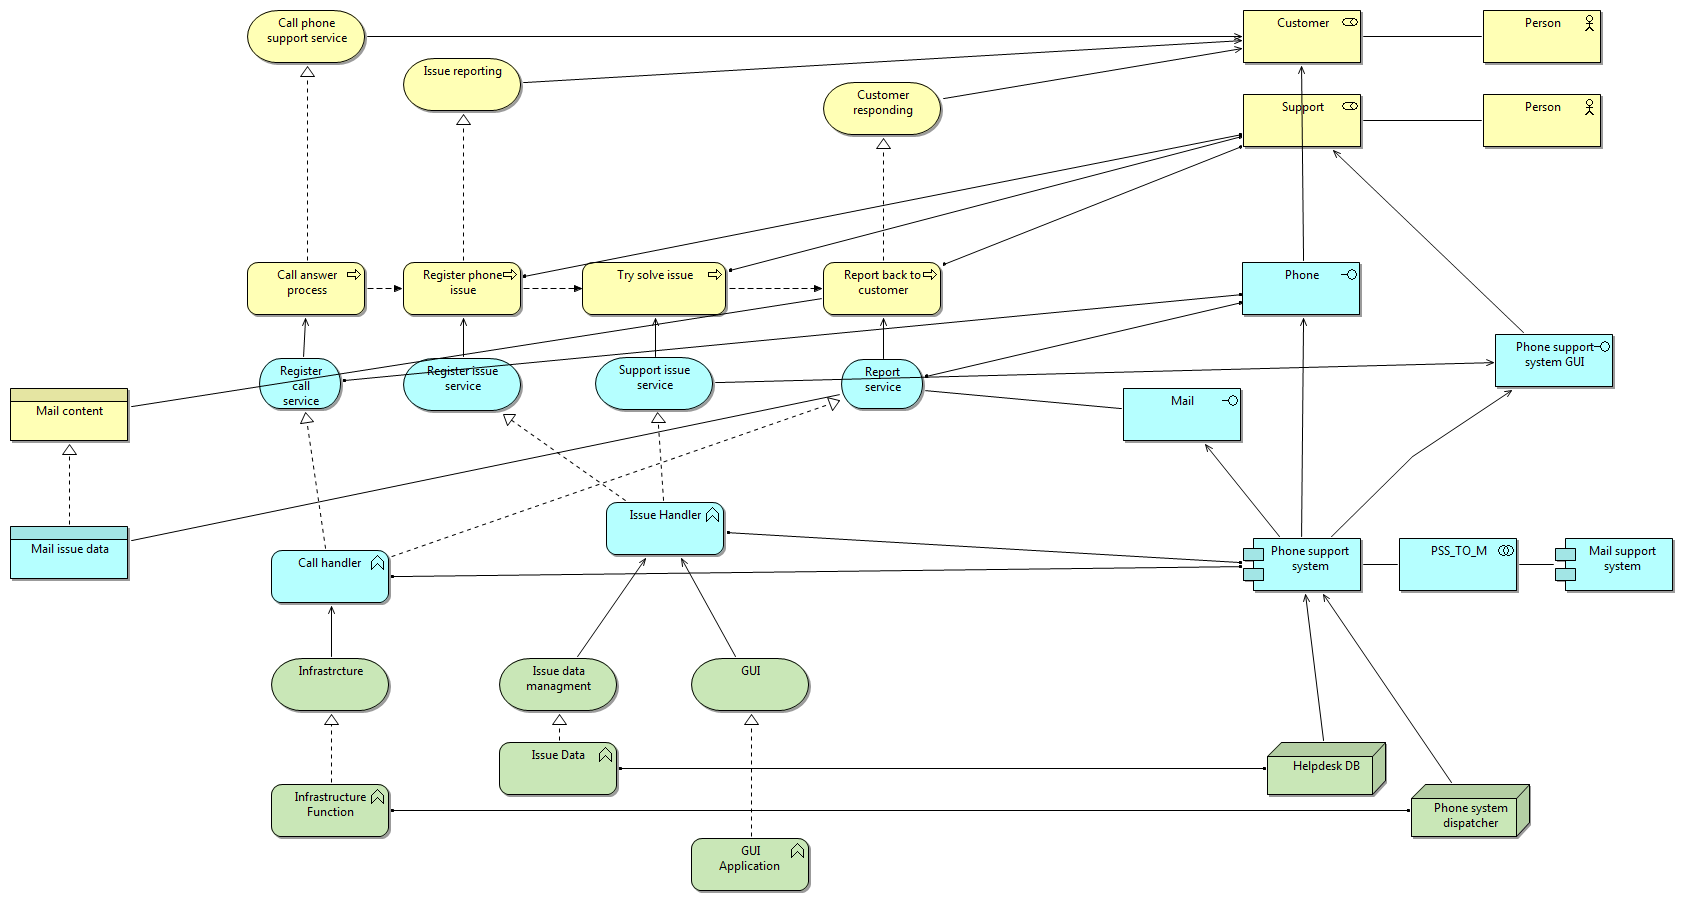
\includegraphics[scale = 0.25]{images/phone.png}}
		\caption{Customer support via telephone (\emph{ArchiMate})}
		\label{fig:archi_phone}
	\end{figure}
\end{center}
%
\paragraph{E-Mail Support}
\label{sec:mail_support}
The customer is able to send an e-mail to get support from J.D.H. Insurance's support team. The e-mail sent to the support team gets registered in the mail support system for help desk team to try solve. When the issue is handled the employee handling the issue sends an e-mail back to the customer including the results from the investigation. Figure 5 shows the services available to the customer and what processes the support team executes to enable e-mail support. This process is shown in \fref{fig:archi_mail}.
\begin{center}
	\begin{figure}[H]
		\centering
		\setlength\fboxsep{7pt}
		\setlength\fboxrule{0.5pt}
		\fbox{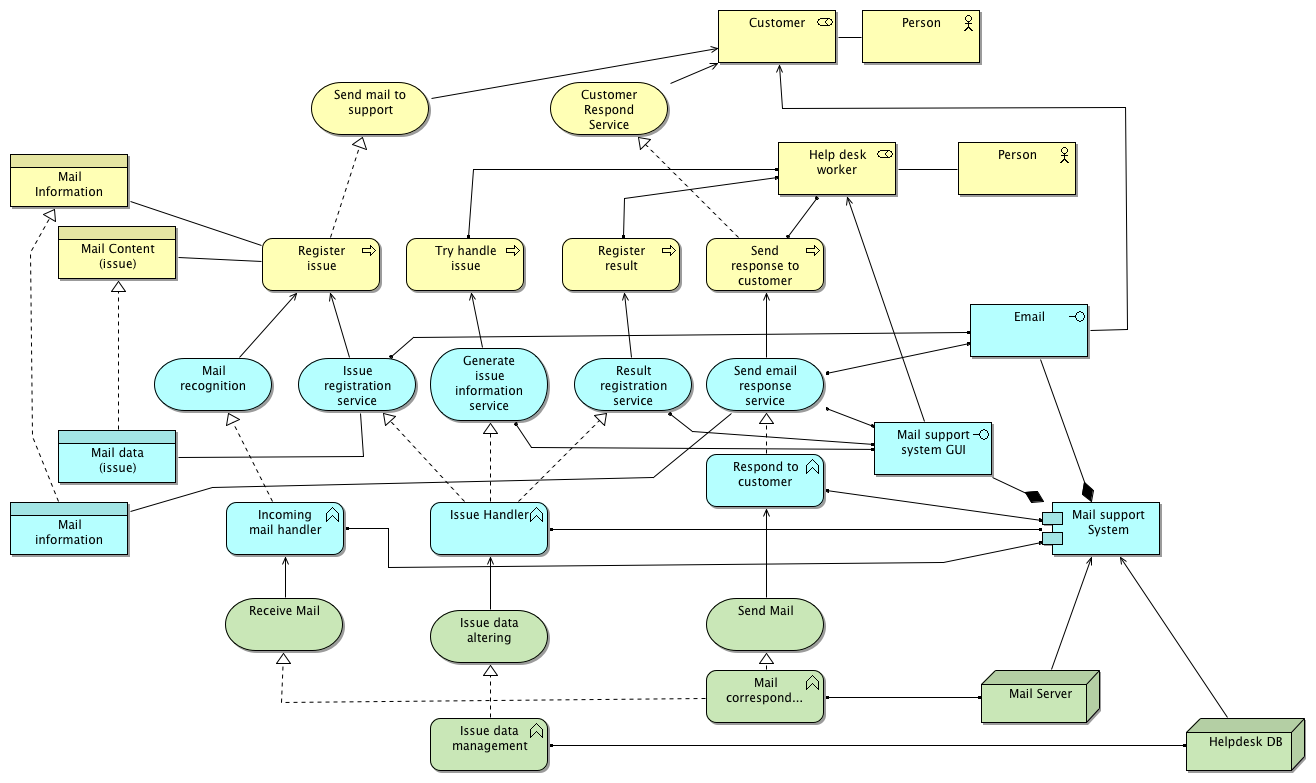
\includegraphics[scale = 0.25]{images/mailsupport.png}}
		\caption{Customer support via e-mail (\emph{ArchiMate})}
		\label{fig:archi_mail}
	\end{figure}
\end{center}
%
\subsection{The As-Is MAP Model}
\label{sec:as_is_map_model}
In this section we depict the different business processes translated to MAP based on the ArchiMate models presented earlier in the report. The following figures (\ref{fig:map_order}-\ref{fig:map_pay}) maps directly to views in the MAP model, thus, the figure depicted in the beginning of the report is all the view merged together. All views can be viewed in the attached iEaat file.
\subsubsection{Order Process MAP Architecture}
\label{sec:order_map}
\begin{center}
	\begin{figure}[H]
		\centering
		\setlength\fboxsep{7pt}
		\setlength\fboxrule{0.5pt}
		\fbox{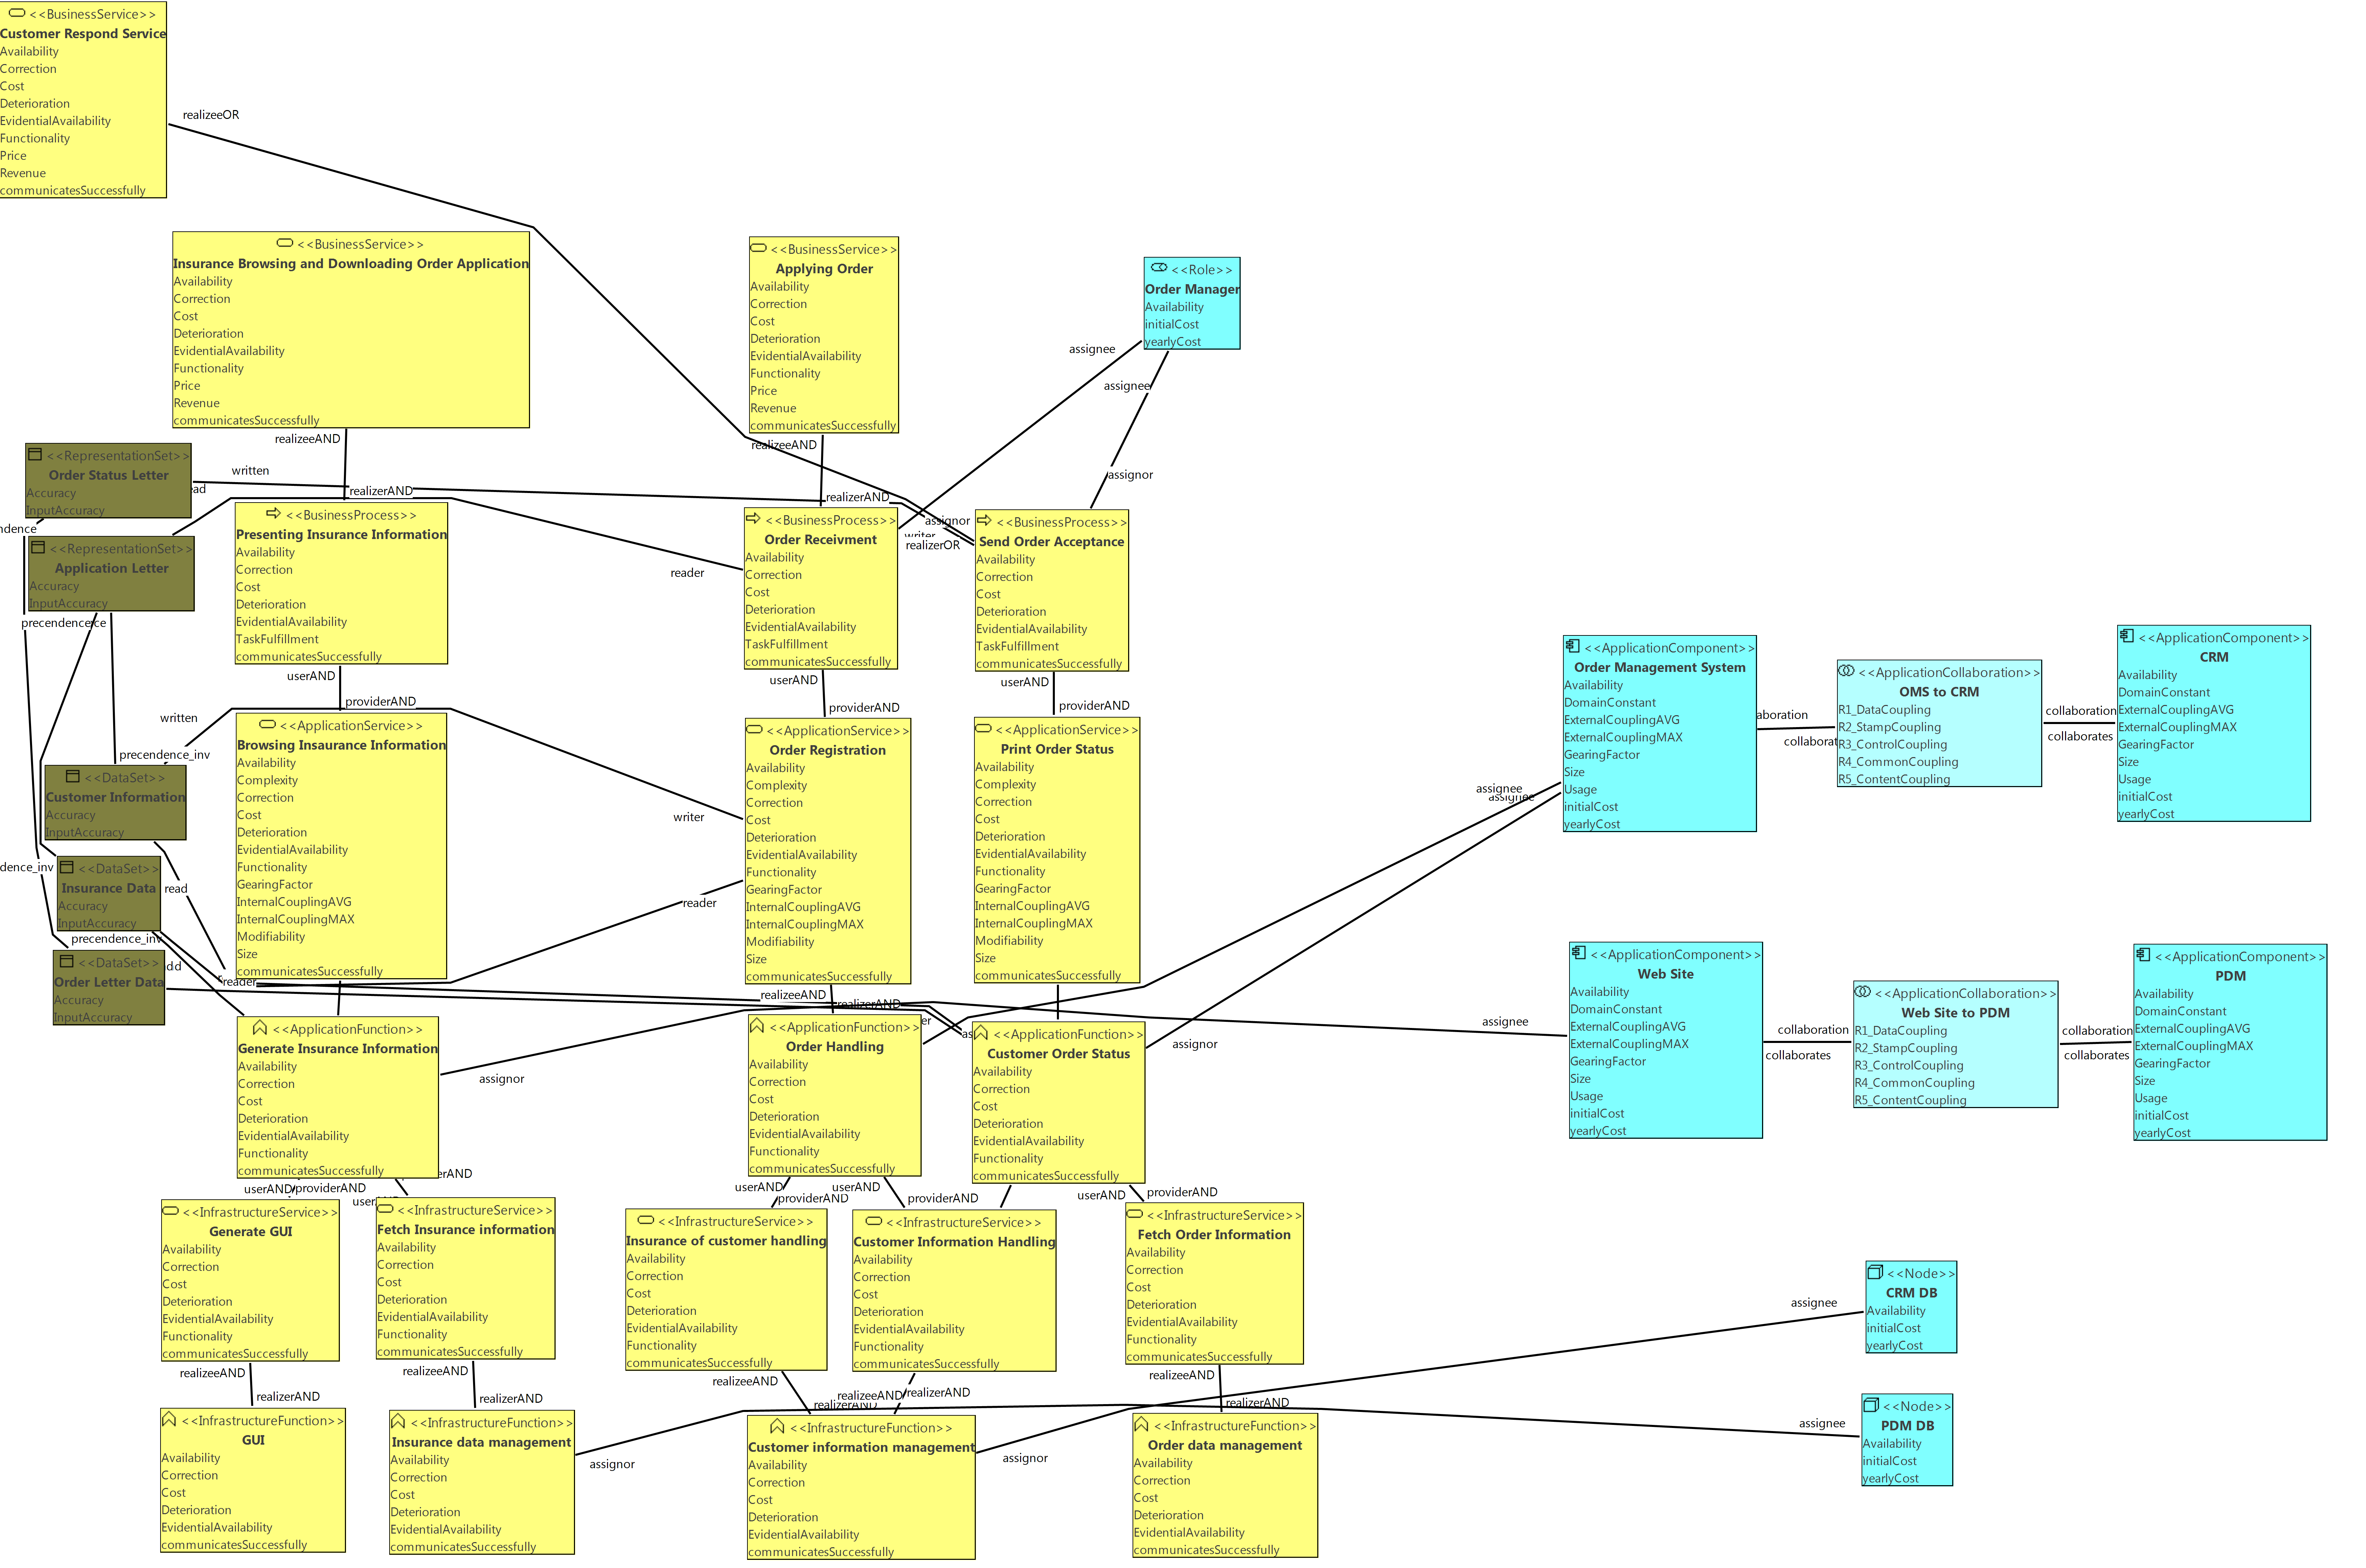
\includegraphics[scale = 0.05]{images/map_order.png}}
		\caption{Order process (\emph{MAP})}
		\label{fig:map_order}
	\end{figure}
\end{center}
%
\subsubsection{Claim Process MAP Architecture}
\label{sec:claim_map}
\begin{center}
	\begin{figure}[H]
		\centering
		\setlength\fboxsep{7pt}
		\setlength\fboxrule{0.5pt}
		\fbox{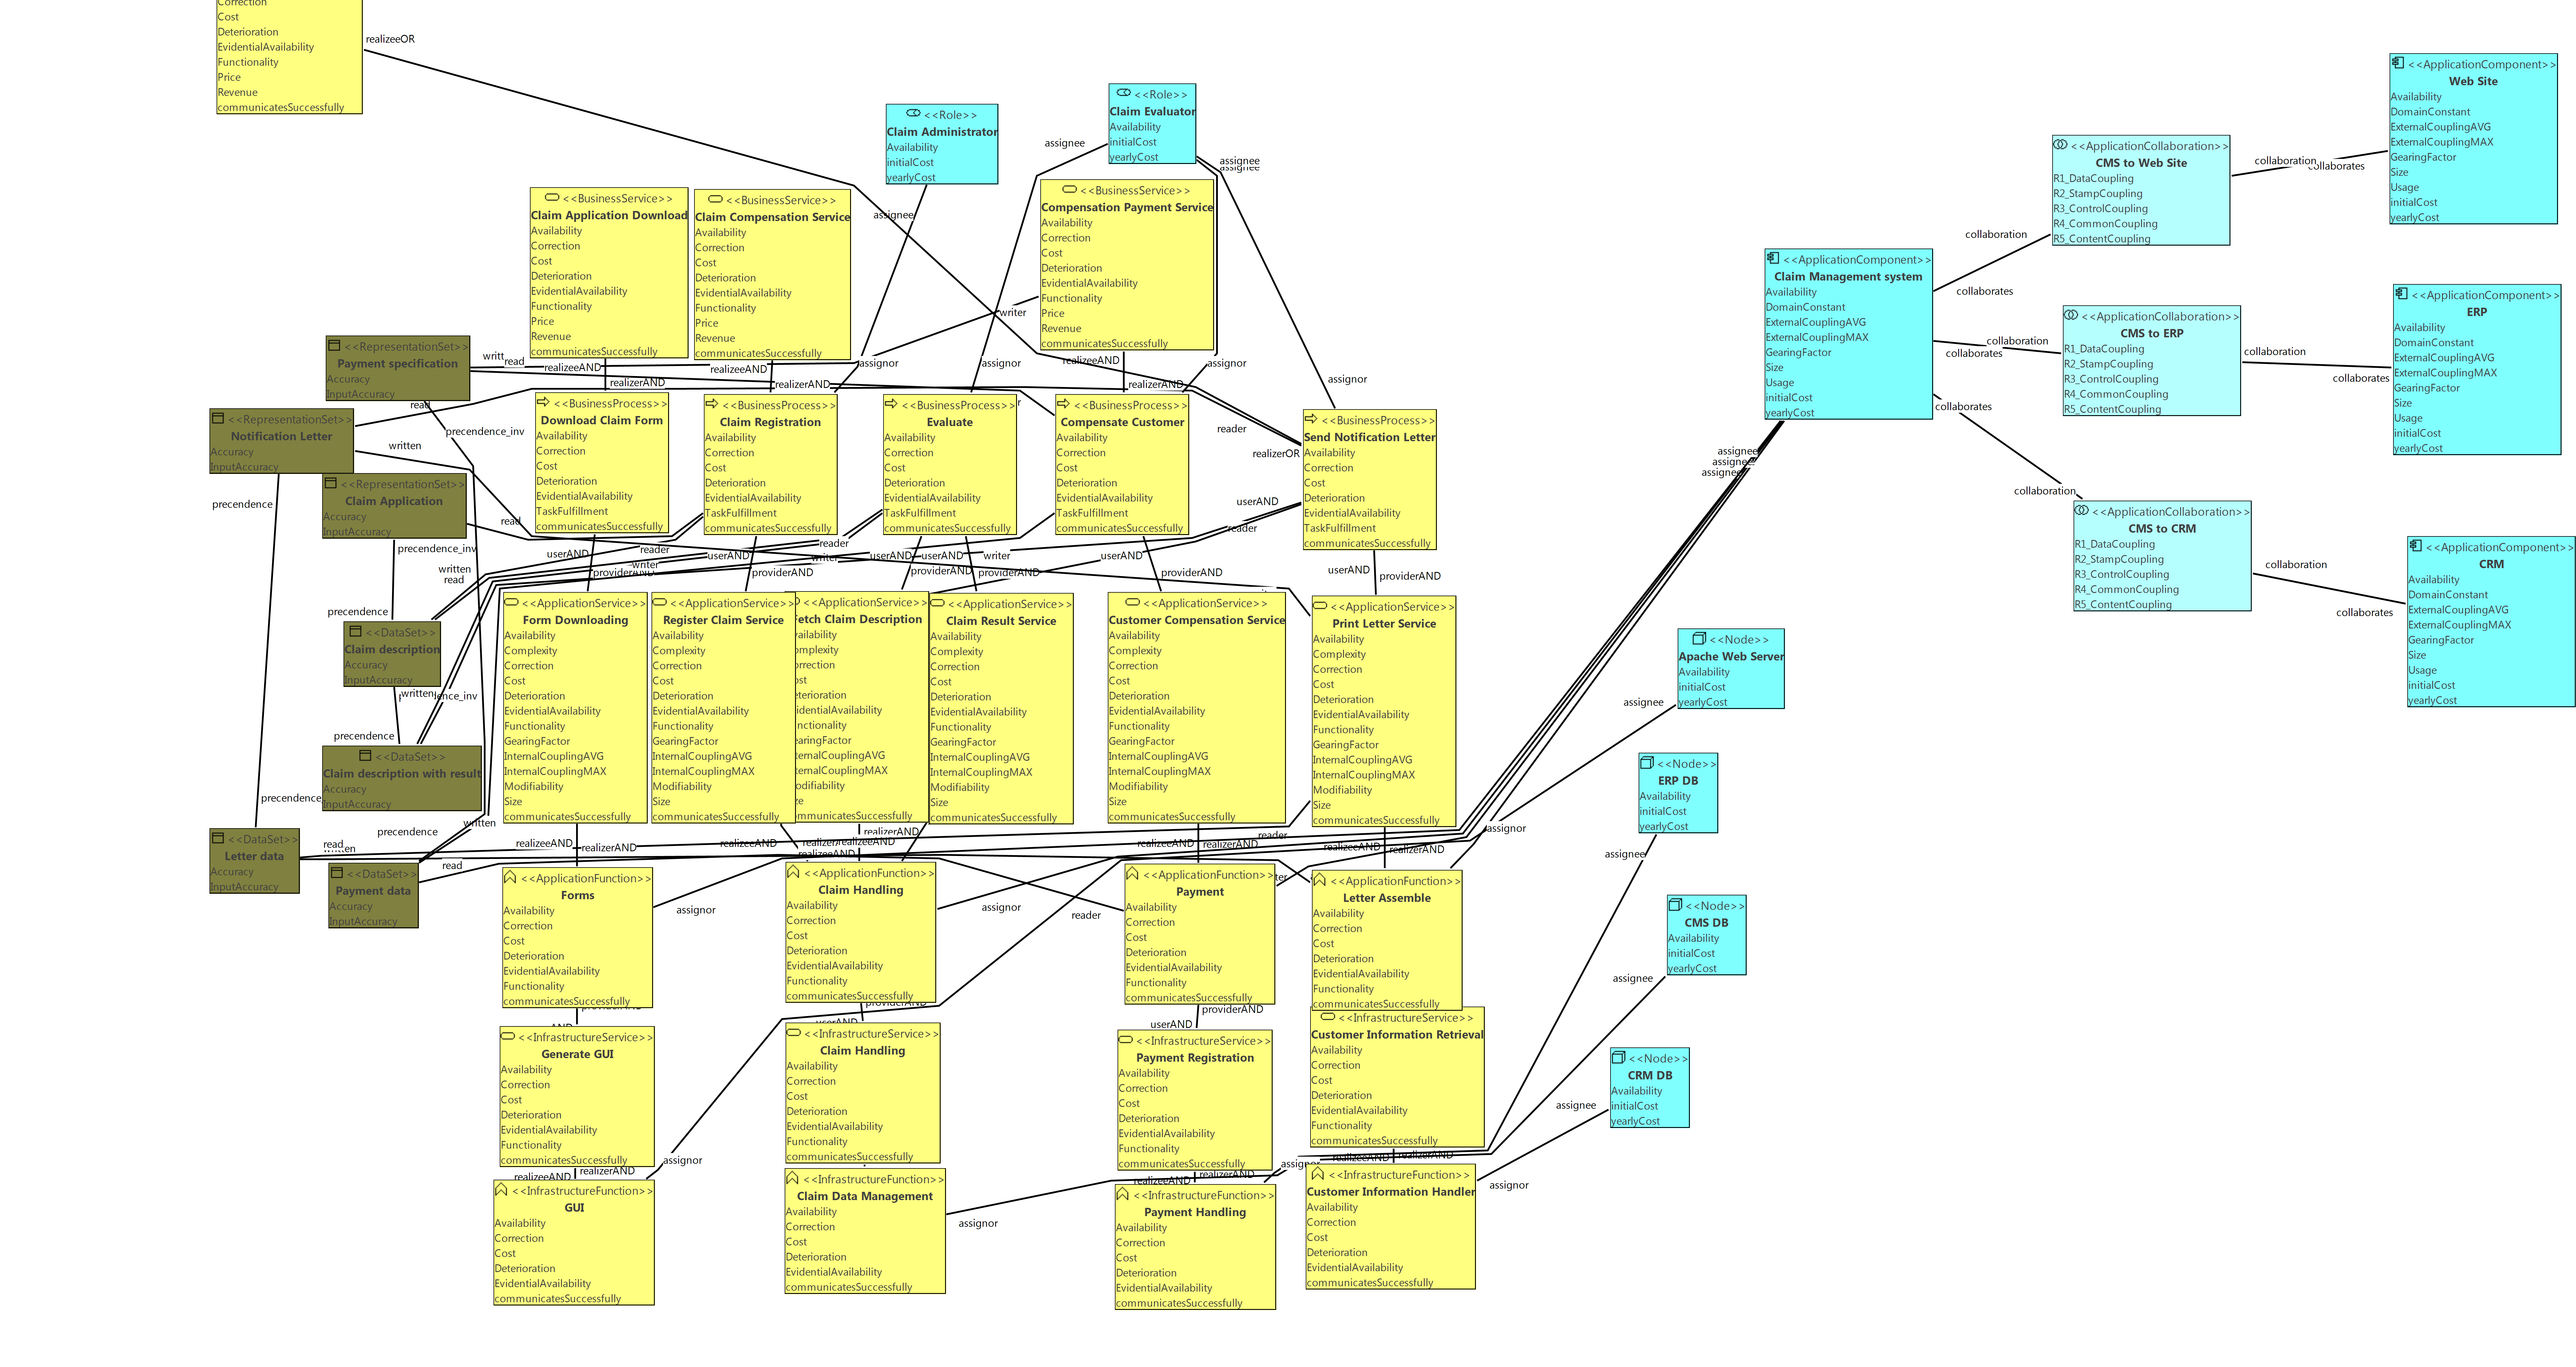
\includegraphics[scale = 0.05]{images/map_claim.png}}
		\caption{Claim process (\emph{MAP})}
		\label{fig:map_claim}
	\end{figure}
\end{center}
%
\subsubsection{E-Mail Support Process MAP Architecture}
\label{sec:mail_map}
\begin{center}
	\begin{figure}[H]
		\centering
		\setlength\fboxsep{7pt}
		\setlength\fboxrule{0.5pt}
		\fbox{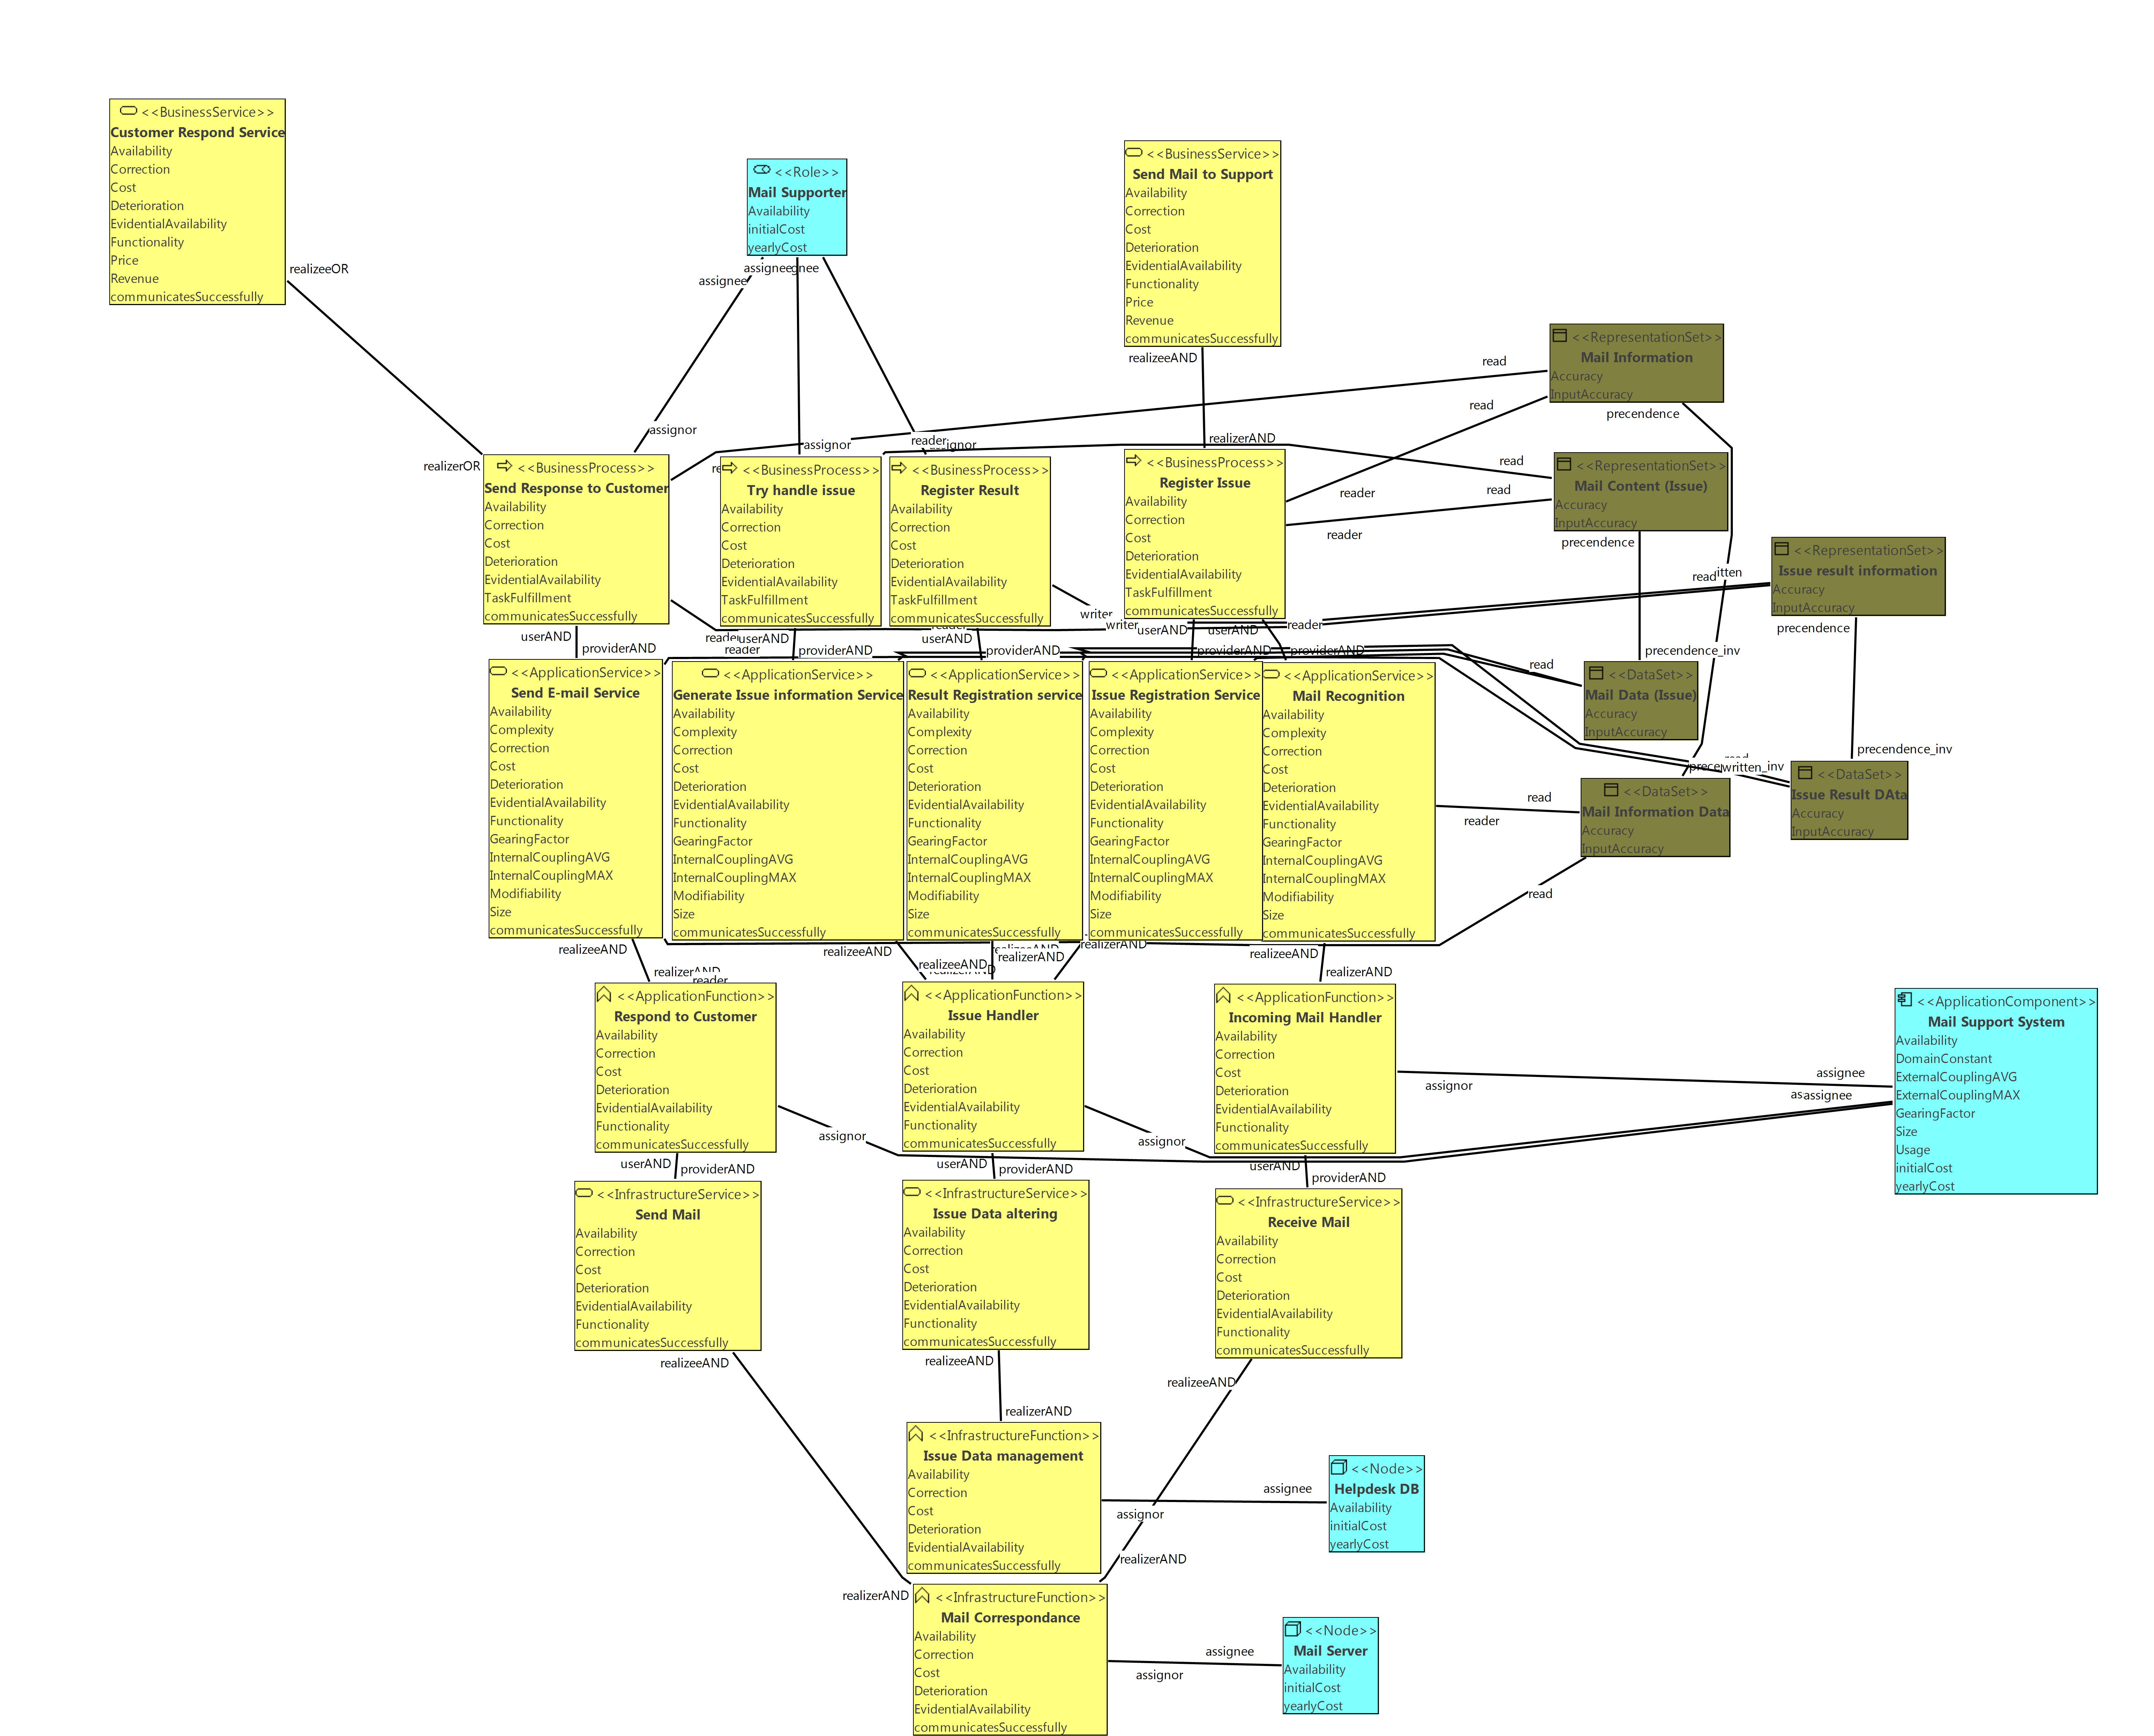
\includegraphics[scale = 0.05]{images/map_mail.png}}
		\caption{Mail process (\emph{MAP})}
		\label{fig:map_mail}
	\end{figure}
\end{center}
%
\subsubsection{Phone Support Process MAP Architecture}
\label{sec:phone_map}
\begin{center}
	\begin{figure}[H]
		\centering
		\setlength\fboxsep{7pt}
		\setlength\fboxrule{0.5pt}
		\fbox{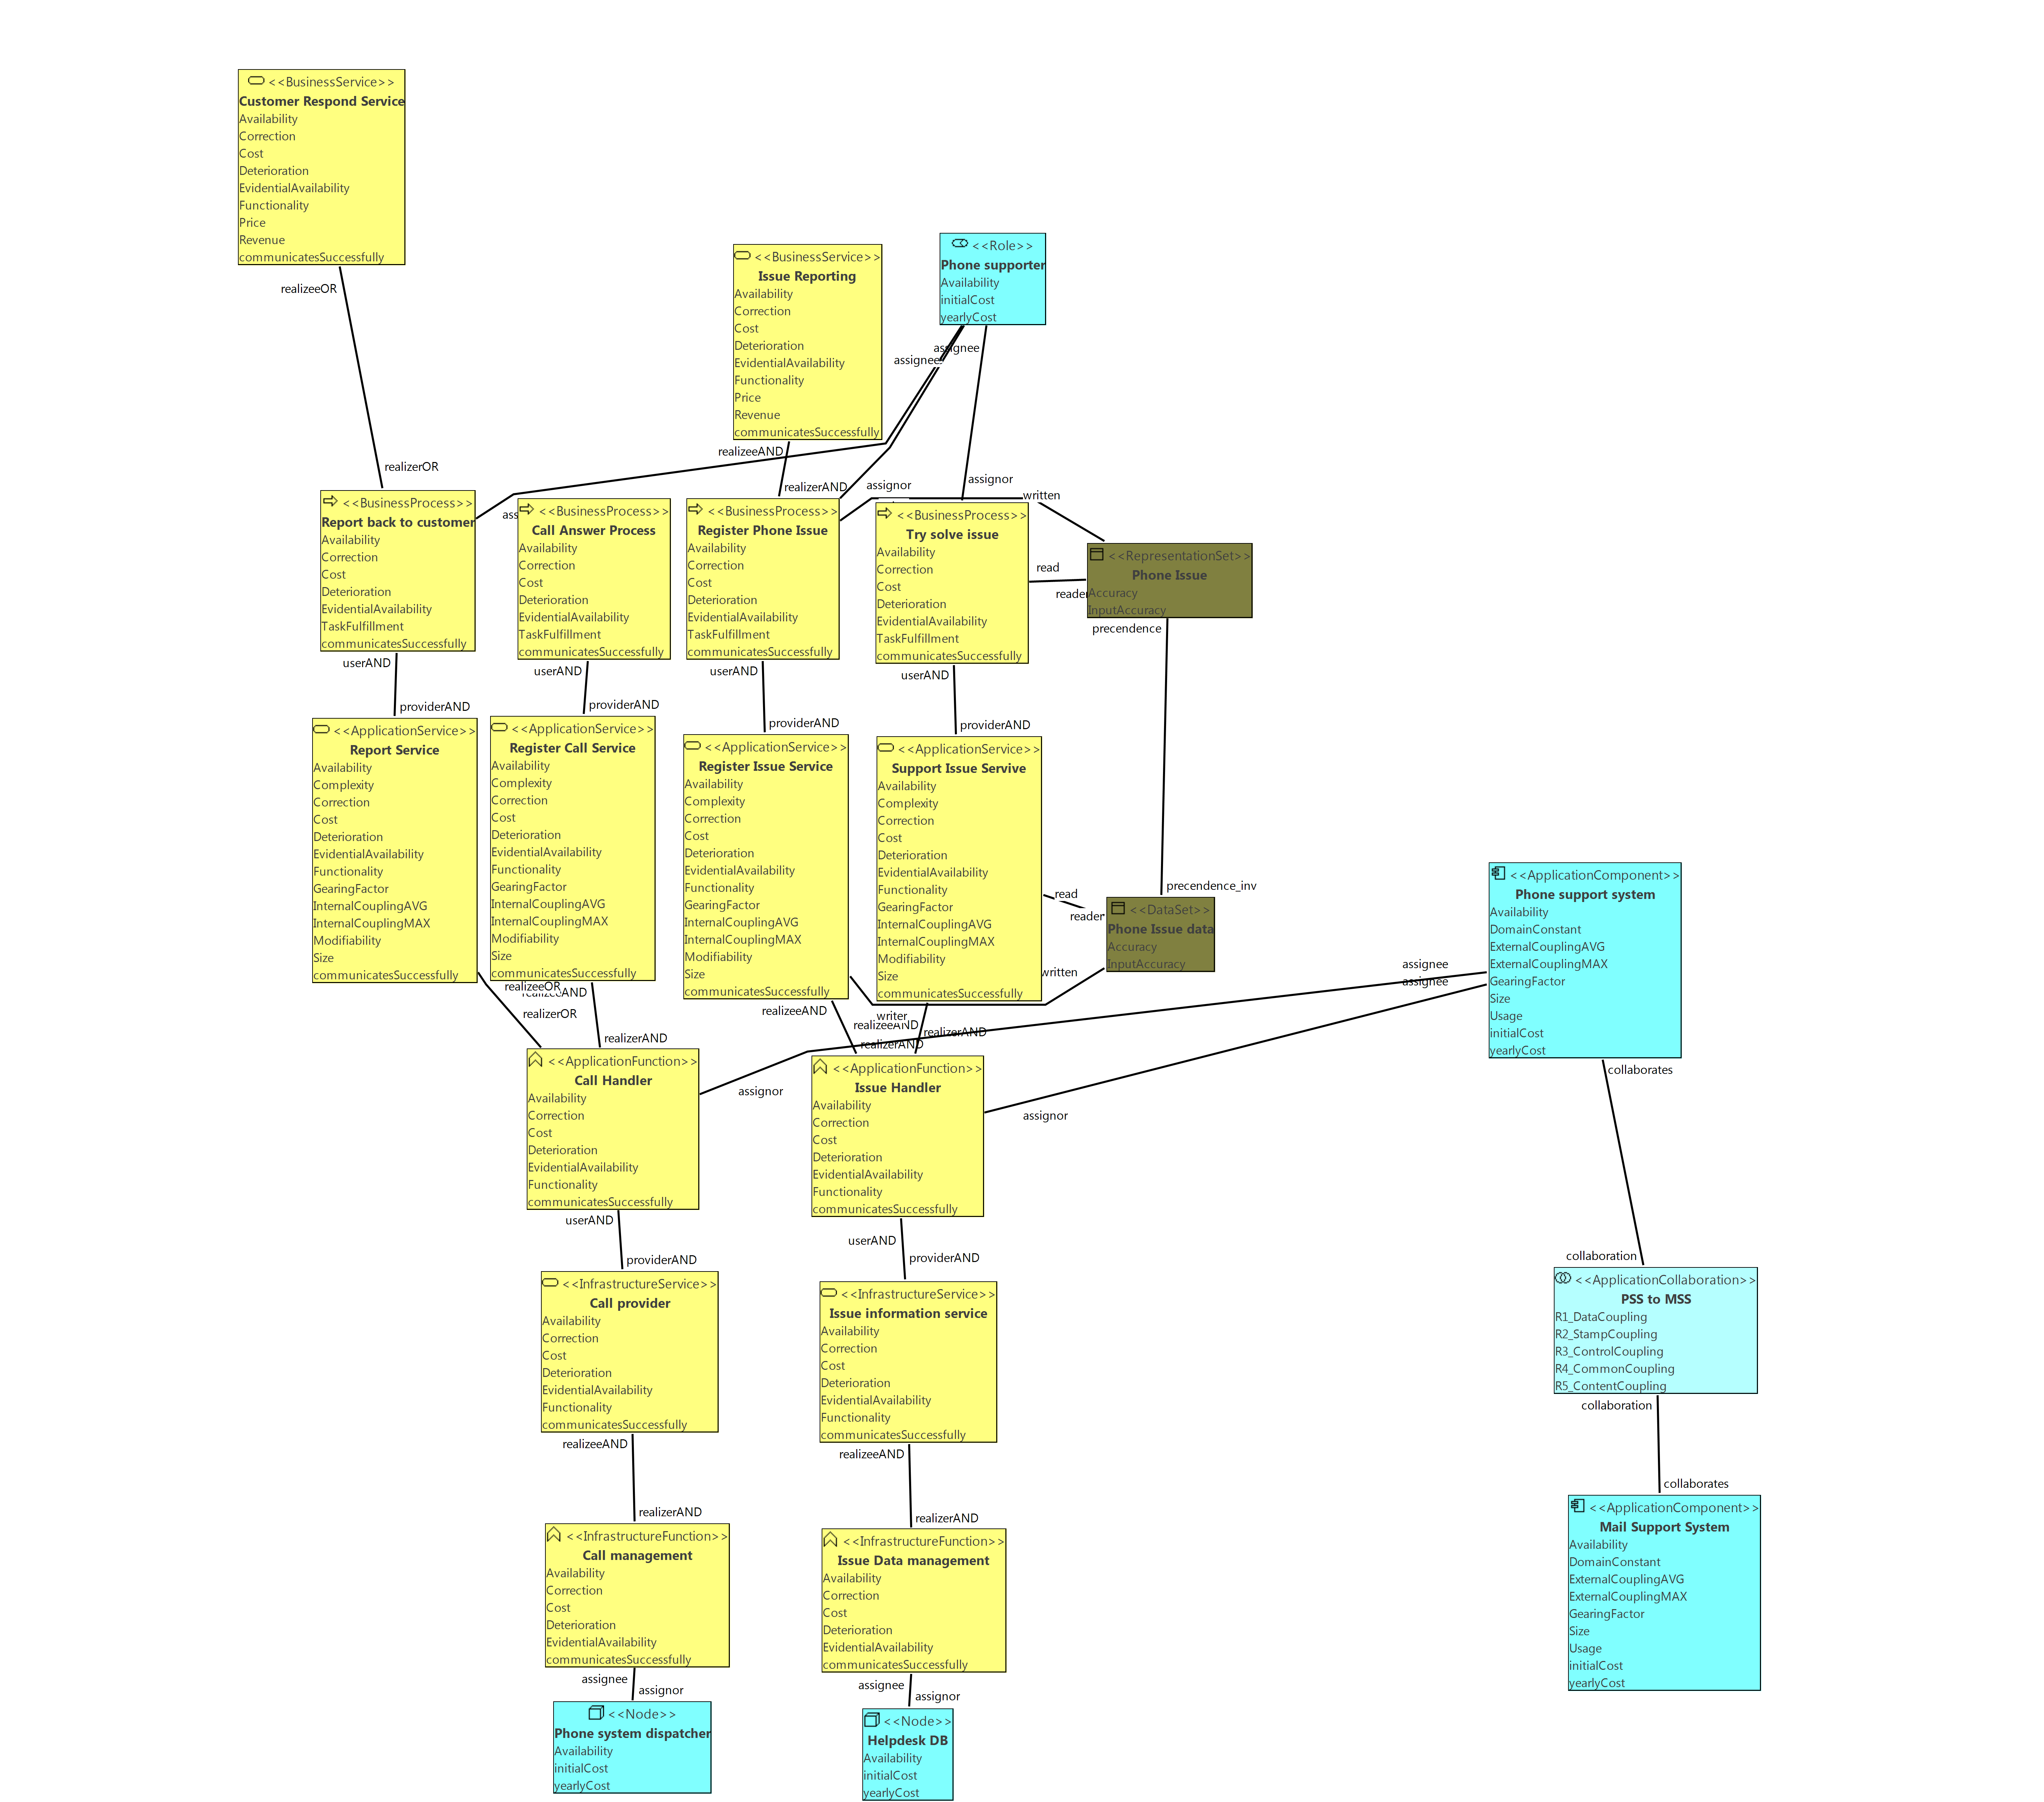
\includegraphics[scale = 0.05]{images/map_phone.png}}
		\caption{Phone process (\emph{MAP})}
		\label{fig:map_phone}
	\end{figure}
\end{center}
%
\subsubsection{Payment Process MAP Architecture}
\label{sec:phone_map}
\begin{center}
	\begin{figure}[H]
		\centering
		\setlength\fboxsep{7pt}
		\setlength\fboxrule{0.5pt}
		\fbox{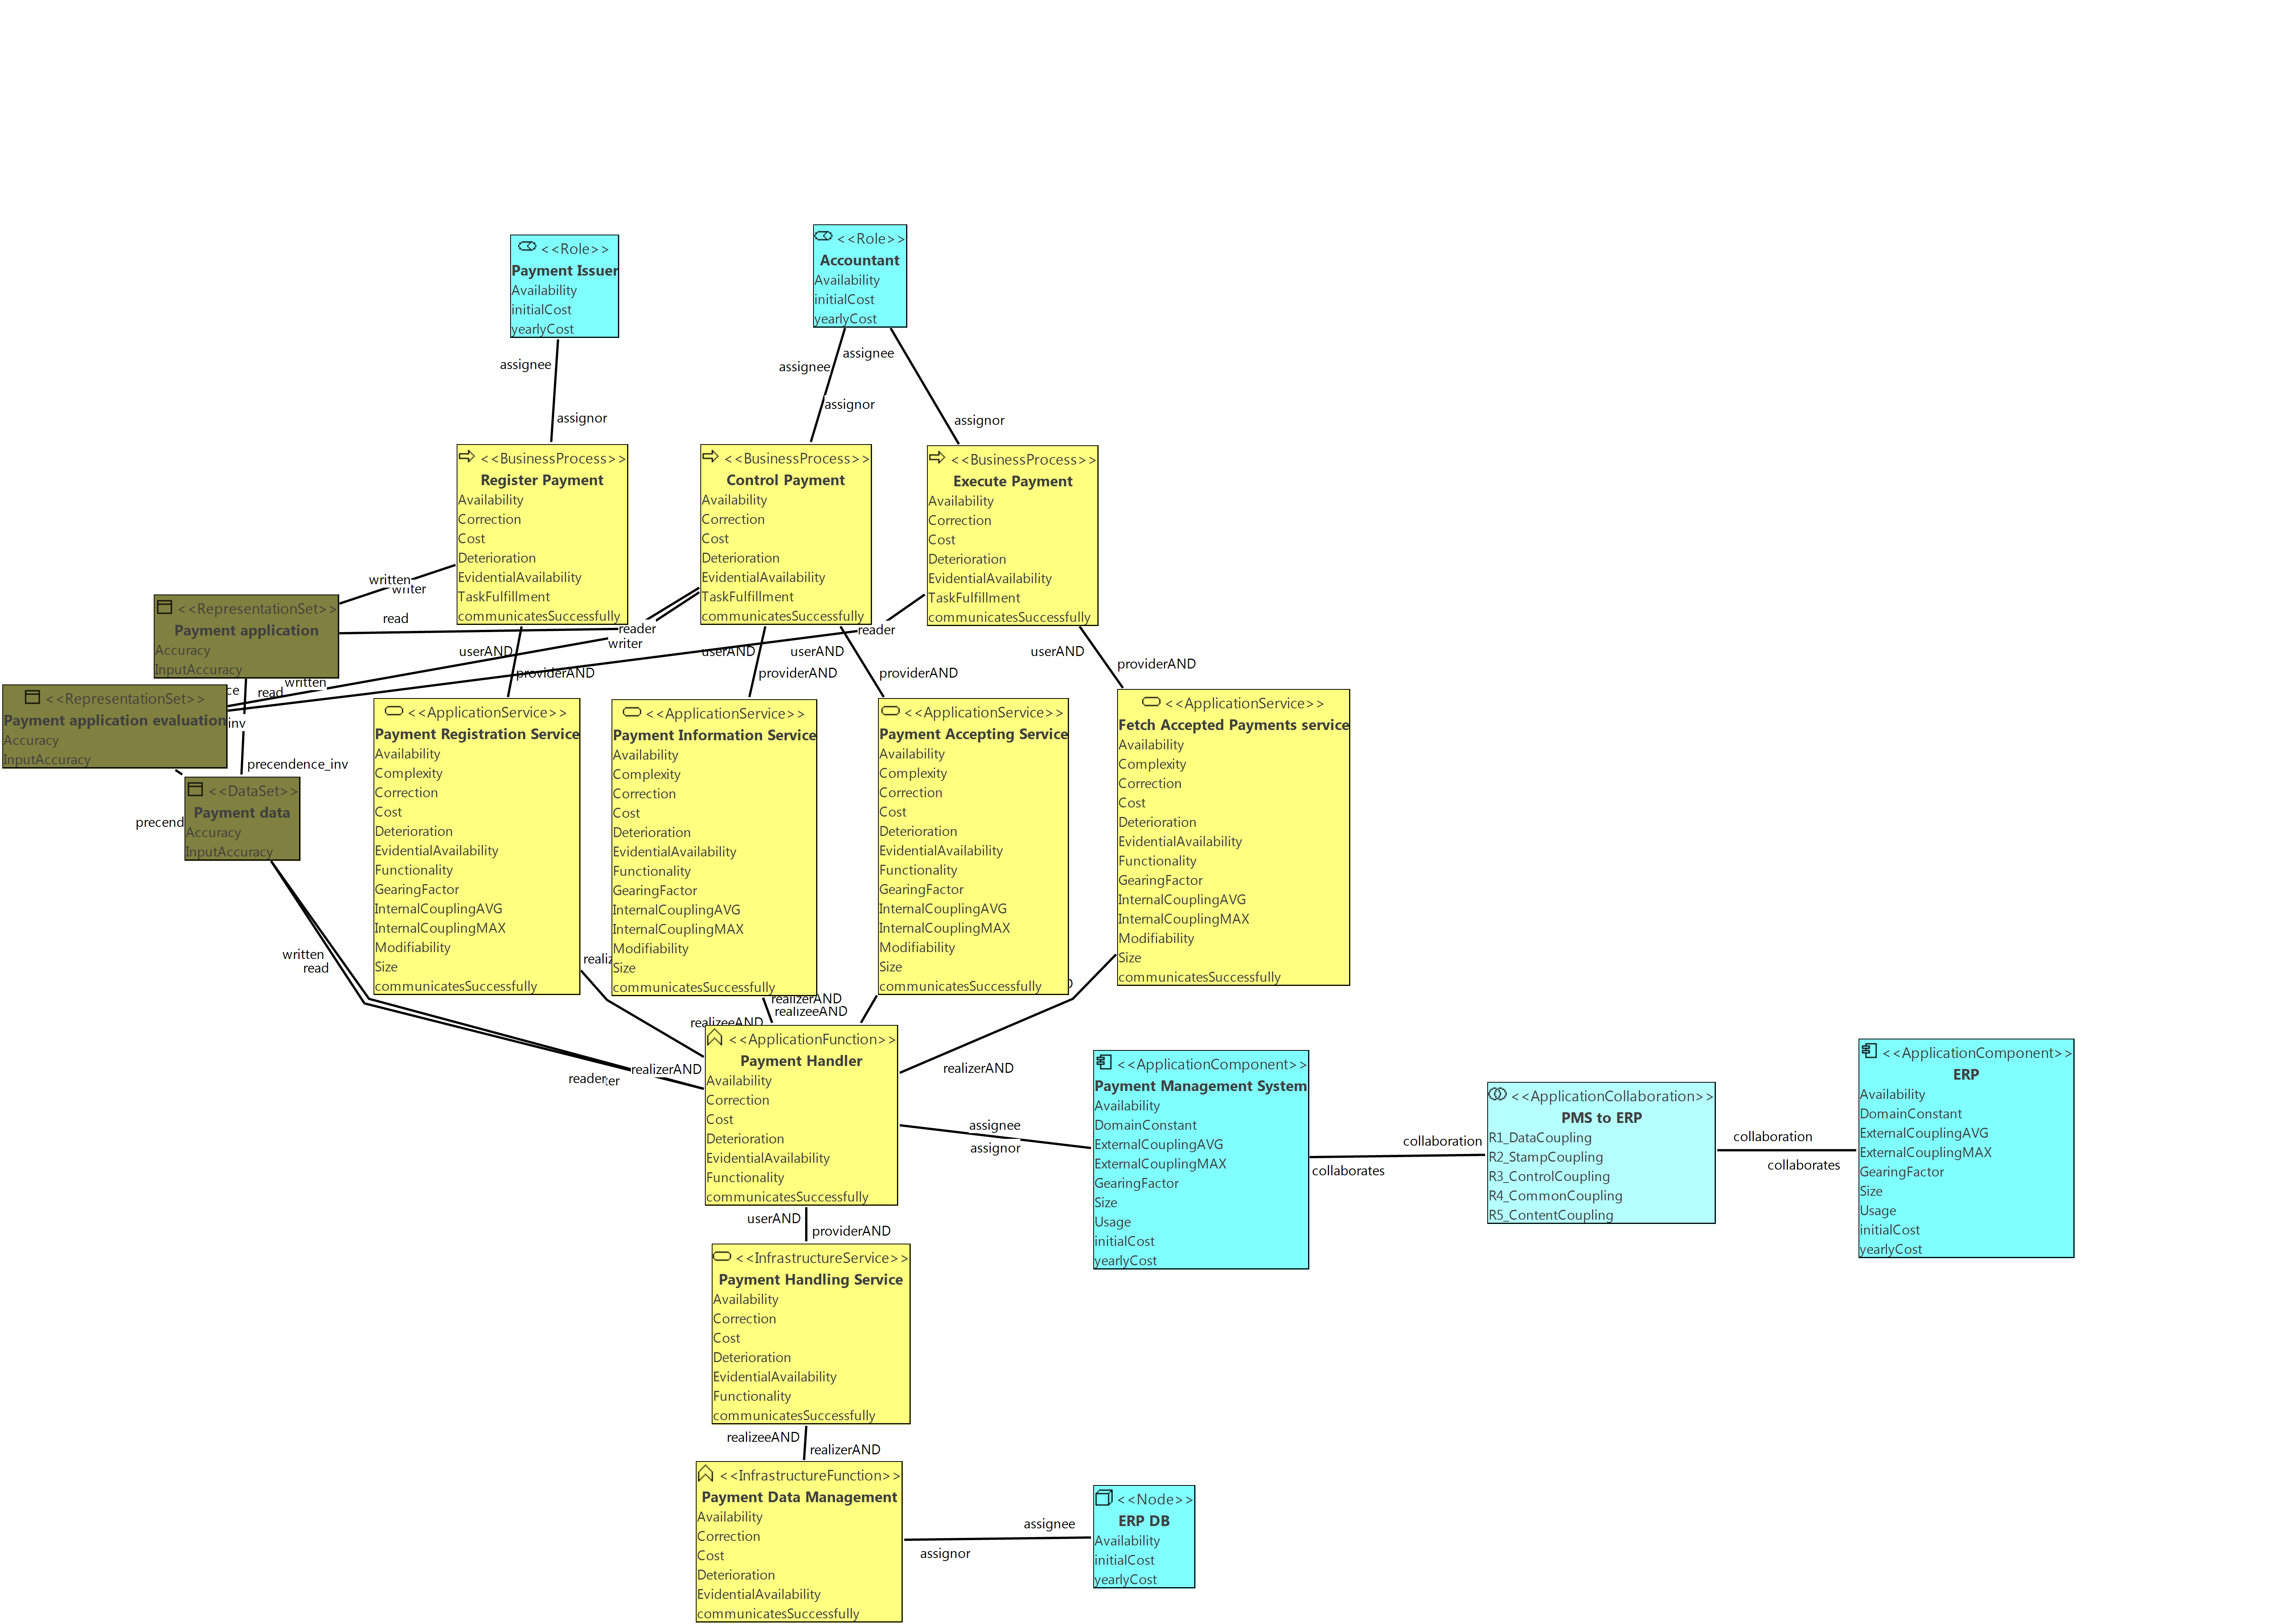
\includegraphics[scale = 0.05]{images/map_pay.png}}
		\caption{Payment process (\emph{MAP})}
		\label{fig:map_pay}
	\end{figure}
\end{center}
%
\subsection{MAP Analysis}
\label{sec:map_analysis}
This section contains analysis of segments of the As-Is MAP model, with respect to MAP attributes, where potential change could be made to reach the vision of the company.
\subsubsection{Claim Registration - Data accuracy}
\label{sec:claim_analysis}
The claim registration service which J.D.H. Insurance provide to the customers they insure has a critical point where it is important that the accuracy of the claims application maintain, that is when the claim administrator receives the claim application from an insurant and registers it into the claim management system. For J.D.H. Insurance to ensure that no information is lost in this process it is vital to analyze the data accuracy of it to see if it can be improved by a new architecture providing higher accuracy. The analyze is done by using the following view, displayed in \fref{fig:map_claim_data}.
\begin{center}
	\begin{figure}[H]
		\centering
		\setlength\fboxsep{7pt}
		\setlength\fboxrule{0.5pt}
		\fbox{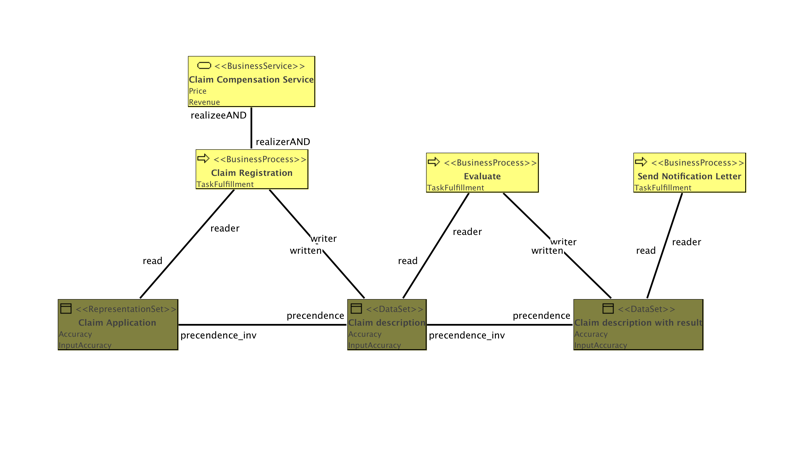
\includegraphics[scale = 0.35]{images/map_claim_data.png}}
		\caption{Data accuracy for the Claim data from received application to the evaluated claim object in the claim management system (\emph{MAP})}
		\label{fig:map_claim_data}
	\end{figure}
\end{center}
The claim application is sent by the insurant to the company and the input accuracy of the application can be assumed to be very high, 0.99. The application is processed by the claim administrator in the claim registration process and the translation from the paper application to the digital description tend to create loss of information, the input accuracy of this is 0.80. The evaluator then reads this description and extends it with an answer, this extension has an input accuracy of 0.95.\\\\
%
This results in a total accuracy loss of 0.81 which seems like a low value for a company evaluating information provided by their customers and which aim to provide the best insurances.
%
\subsubsection{Support - Service Availability}
\label{sec:support_analysis}
One of J.D.H. Insurance visions is to provide the best support for their customers. One important aspect of this support is the availability of the support. Clearly the access points for the support functions need to be available to the customers if they should be able to contact J.D.H. Insurance. An analysis of the availability of the access points of both the support architectures would then be of value for J.D.H. Insurance, and to evaluate what improvements that could be done to increase the availability of these services. The following view, \fref{fig:map_support_phone_availability}, shows the service of calling to the phone support and analyzes its availability to the customers.
\begin{center}
	\begin{figure}[H]
		\centering
		\setlength\fboxsep{7pt}
		\setlength\fboxrule{0.5pt}
		\fbox{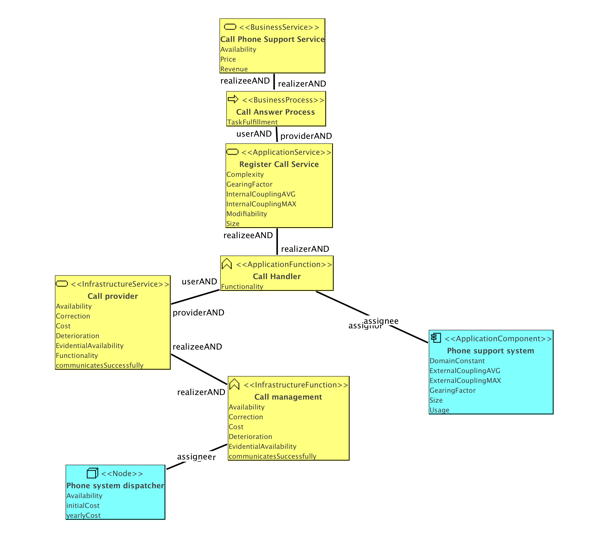
\includegraphics[scale = 0.35]{images/map_support_phone_availability.png}}
		\caption{Service availability of the Phone support access service (\emph{MAP})}
		\label{fig:map_support_phone_availability}
	\end{figure}
\end{center}
The Phone support system has an availability of 0.95. The Phone system dispatcher has an availability of 0.96. The infrastructure function Call management and the infrastructure service call provider has evidential availability of 0.95.\\\\
%
The result of the analysis of these values gives an availability of 0.91 for the service, which is a low value for a service which should be able to compete with other companies similar services.
\begin{center}
	\begin{figure}[H]
		\centering
		\setlength\fboxsep{7pt}
		\setlength\fboxrule{0.5pt}
		\fbox{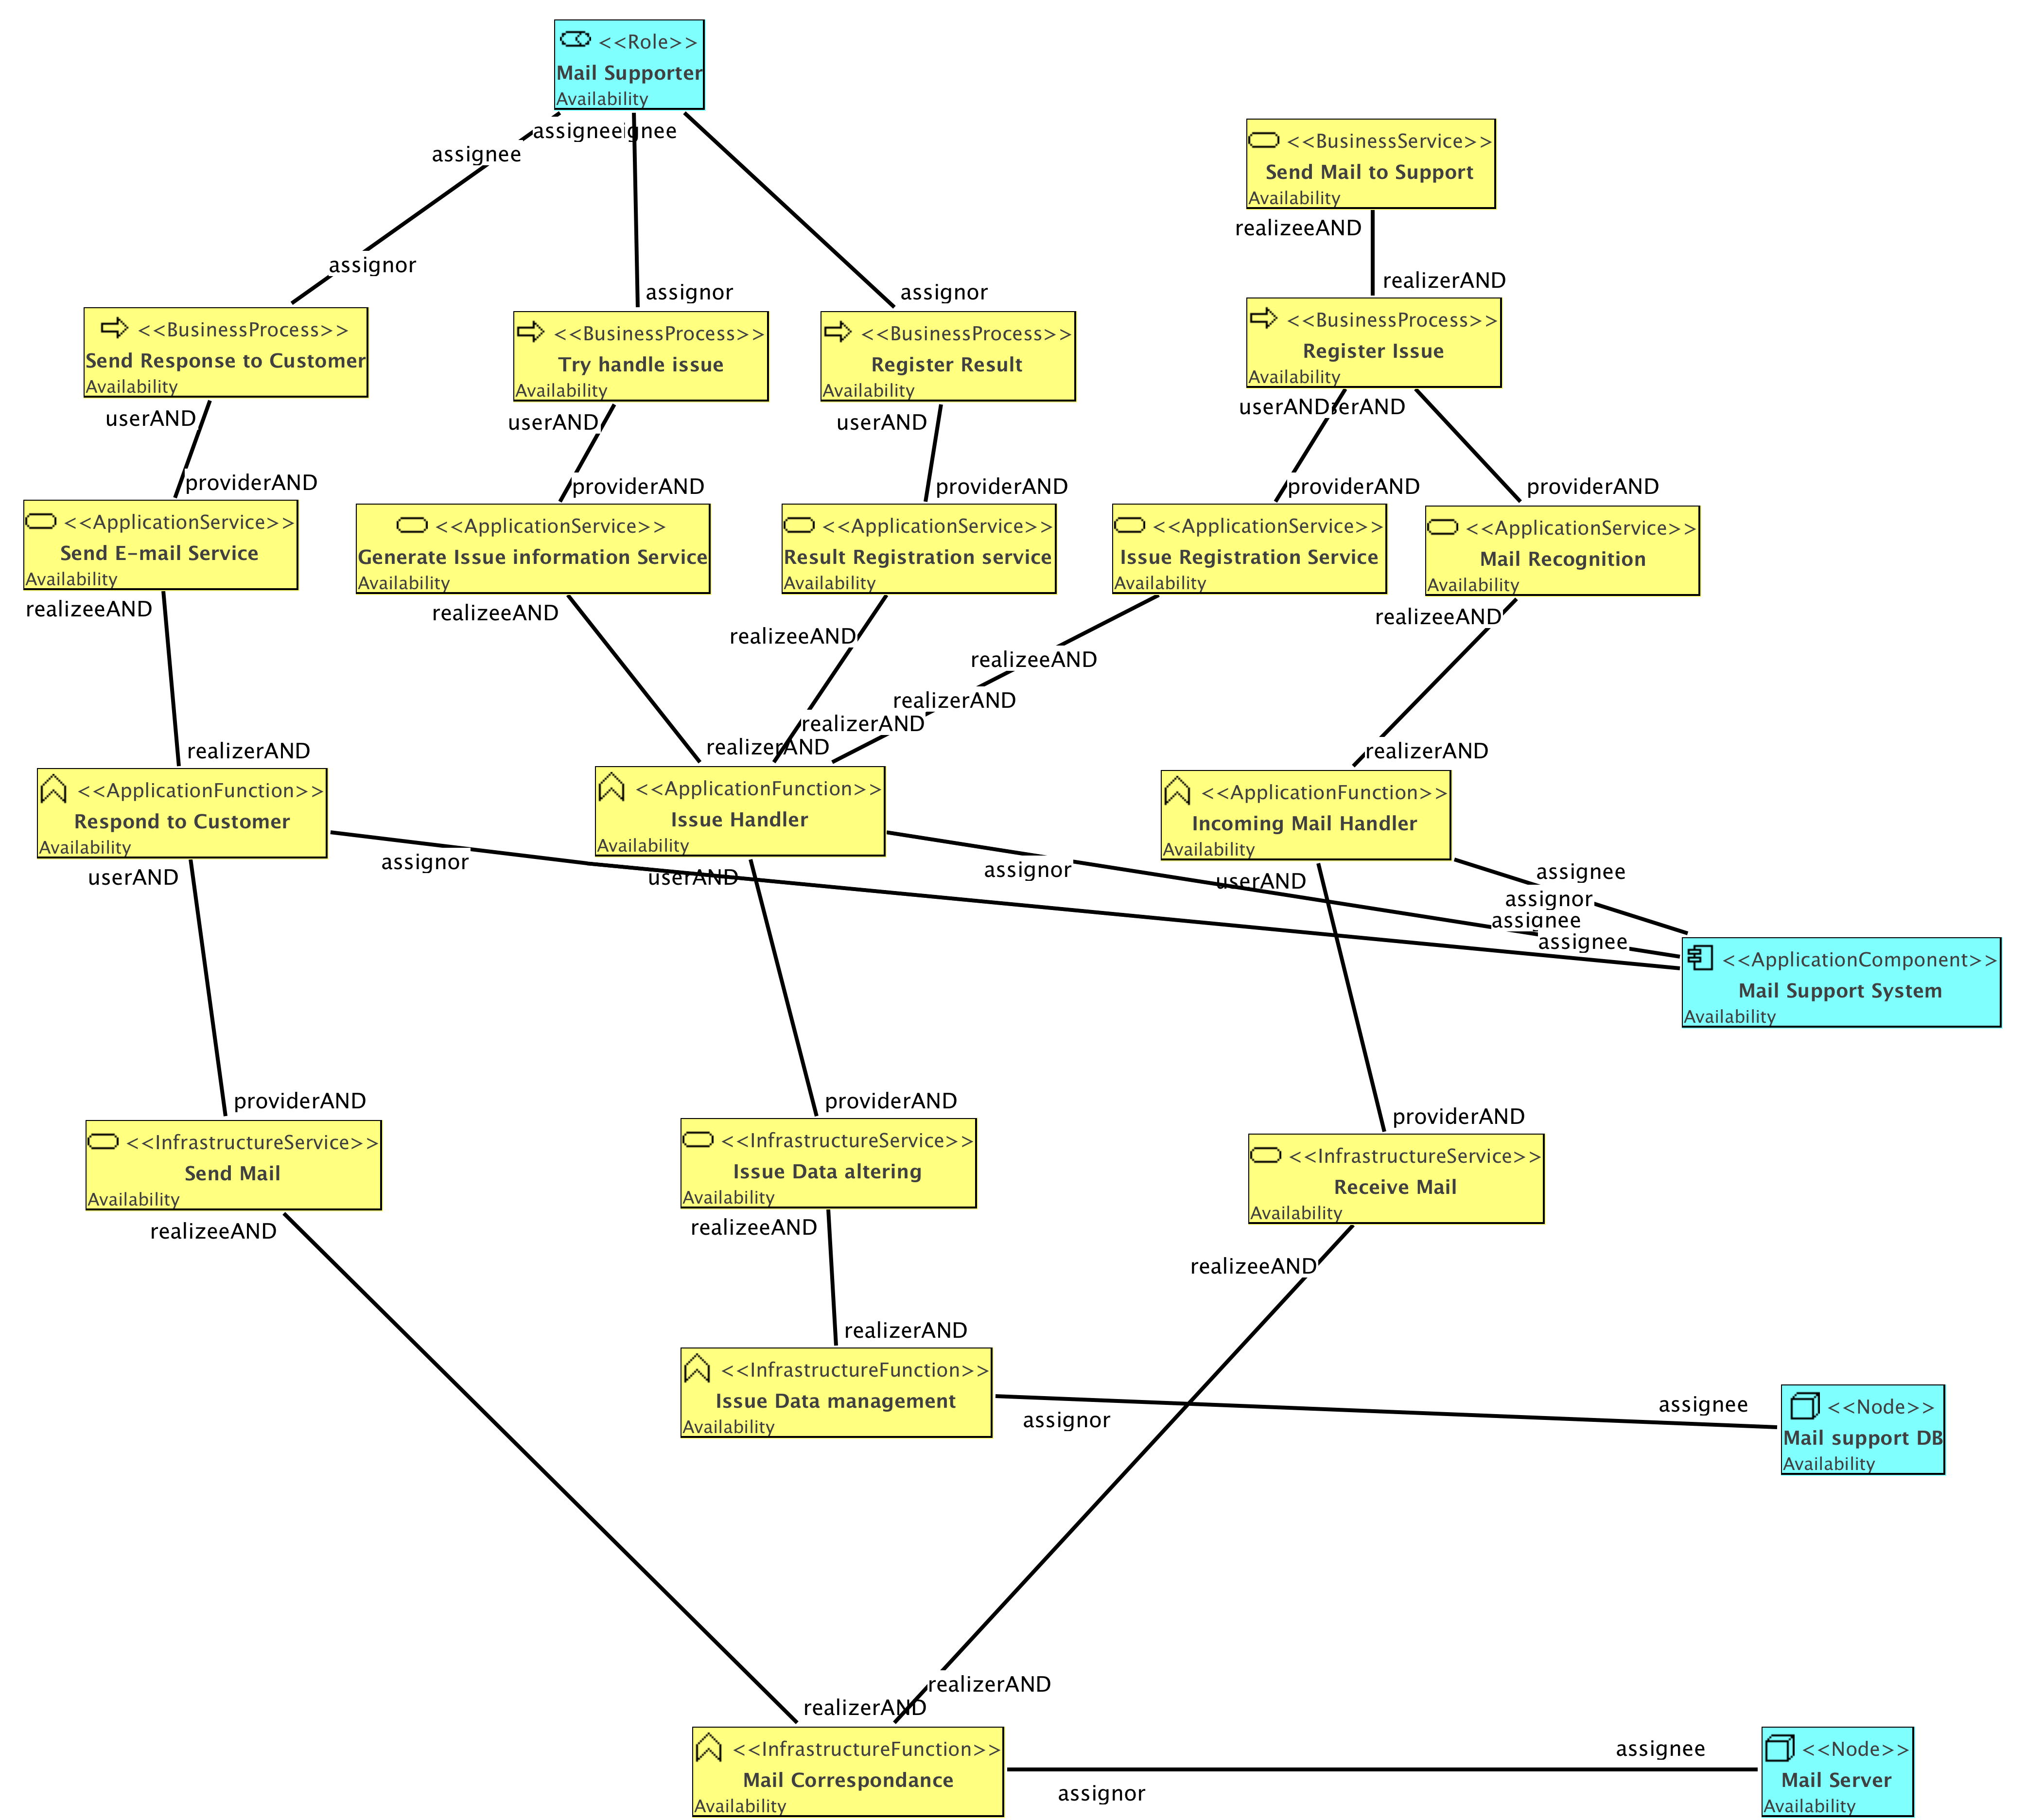
\includegraphics[scale = 0.09]{images/map_support_email_availability.png}}
		\caption{Service availability of the Mail support service (\emph{MAP})}
		\label{fig:map_support_mail_availability}
	\end{figure}
\end{center}
TODO text and tables\\\\
%
\subsubsection{Order Registration and Sending Reports - Cost}
\label{sec:order_analysis}
The registration of order application and sending the order acceptance letter as response are two processes which uses several systems and a role in the company. The role is an Order manager registering and sending acceptance letters. The systems he uses are order management systems, the order management database and the customer relation database. All this systems and the role seems quite costly for such a simple process, and to reach the vision of the company a more cost efficient architecture of these processes would help J.D.H. Insurance to provide better services and insurances. This architecture is interesting to analyze since it would be possible to replace the manager with an automated system and improve the usage of the order management system. The following view, \fref{fig:map_order_cost}, shows the view analyzed for finding cost in the processes which includes the manager.
\begin{center}
	\begin{figure}[H]
		\centering
		\setlength\fboxsep{7pt}
		\setlength\fboxrule{0.5pt}
		\fbox{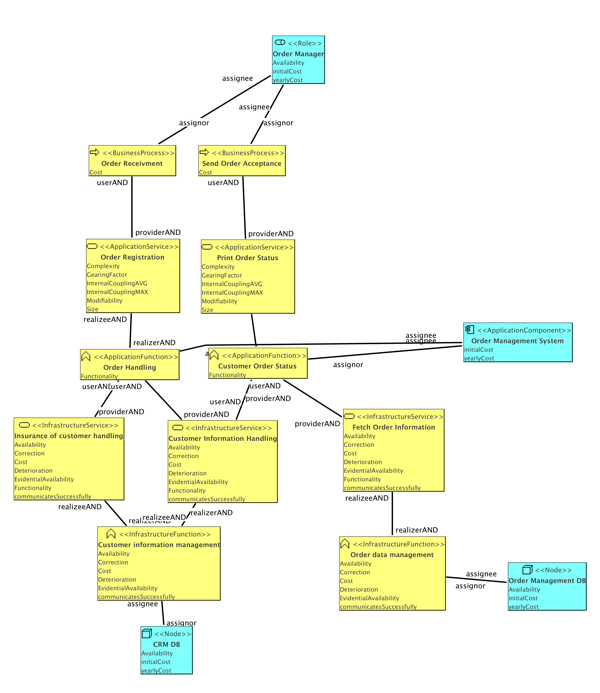
\includegraphics[scale = 0.35]{images/map_order_cost.png}}
		\caption{Cost of the processes "Order Receivement" and "Send Order Acceptance" (\emph{MAP})}
		\label{fig:map_order_cost}
	\end{figure}
\end{center}
The manager is a yearly cost for the company of 500' SEK, that includes salary and recruitment costs etc. The Order management system had an initial cost of 1500' SEK since its a large and complex system and a yearly cost of 300' SEK. The Order management database had an initial cost of 400' SEK and an yearly cost of 100' SEK. The CRM database is the most modern of these systems and was an initial cost of 700' SEK and is a yearly cost of 50' SEK.\\\\
%
The analysis resulted in a cost for the "Order receivement" process of 1525' SEK and a cost for the "Send Order Acceptance" process of 1837500 SEK.
%
\subsubsection{Order Registration - Availability}
\label{sec:order_availability}
In order to achieve maximum customer satisfaction the availability of the order registration service is crucial, as this currently is the sole entry point for customers intending to purchase an insurance. Consequently an increase in order availability could then help mitigate situations where a customer is unable to make an order due to system failure; and potentially missing out in a customer. In \fref{fig:map_order_availability}, the current as-is situation of order registration view is depicted.
\begin{center}
	\begin{figure}[H]
		\centering
		\setlength\fboxsep{7pt}
		\setlength\fboxrule{0.5pt}
		\fbox{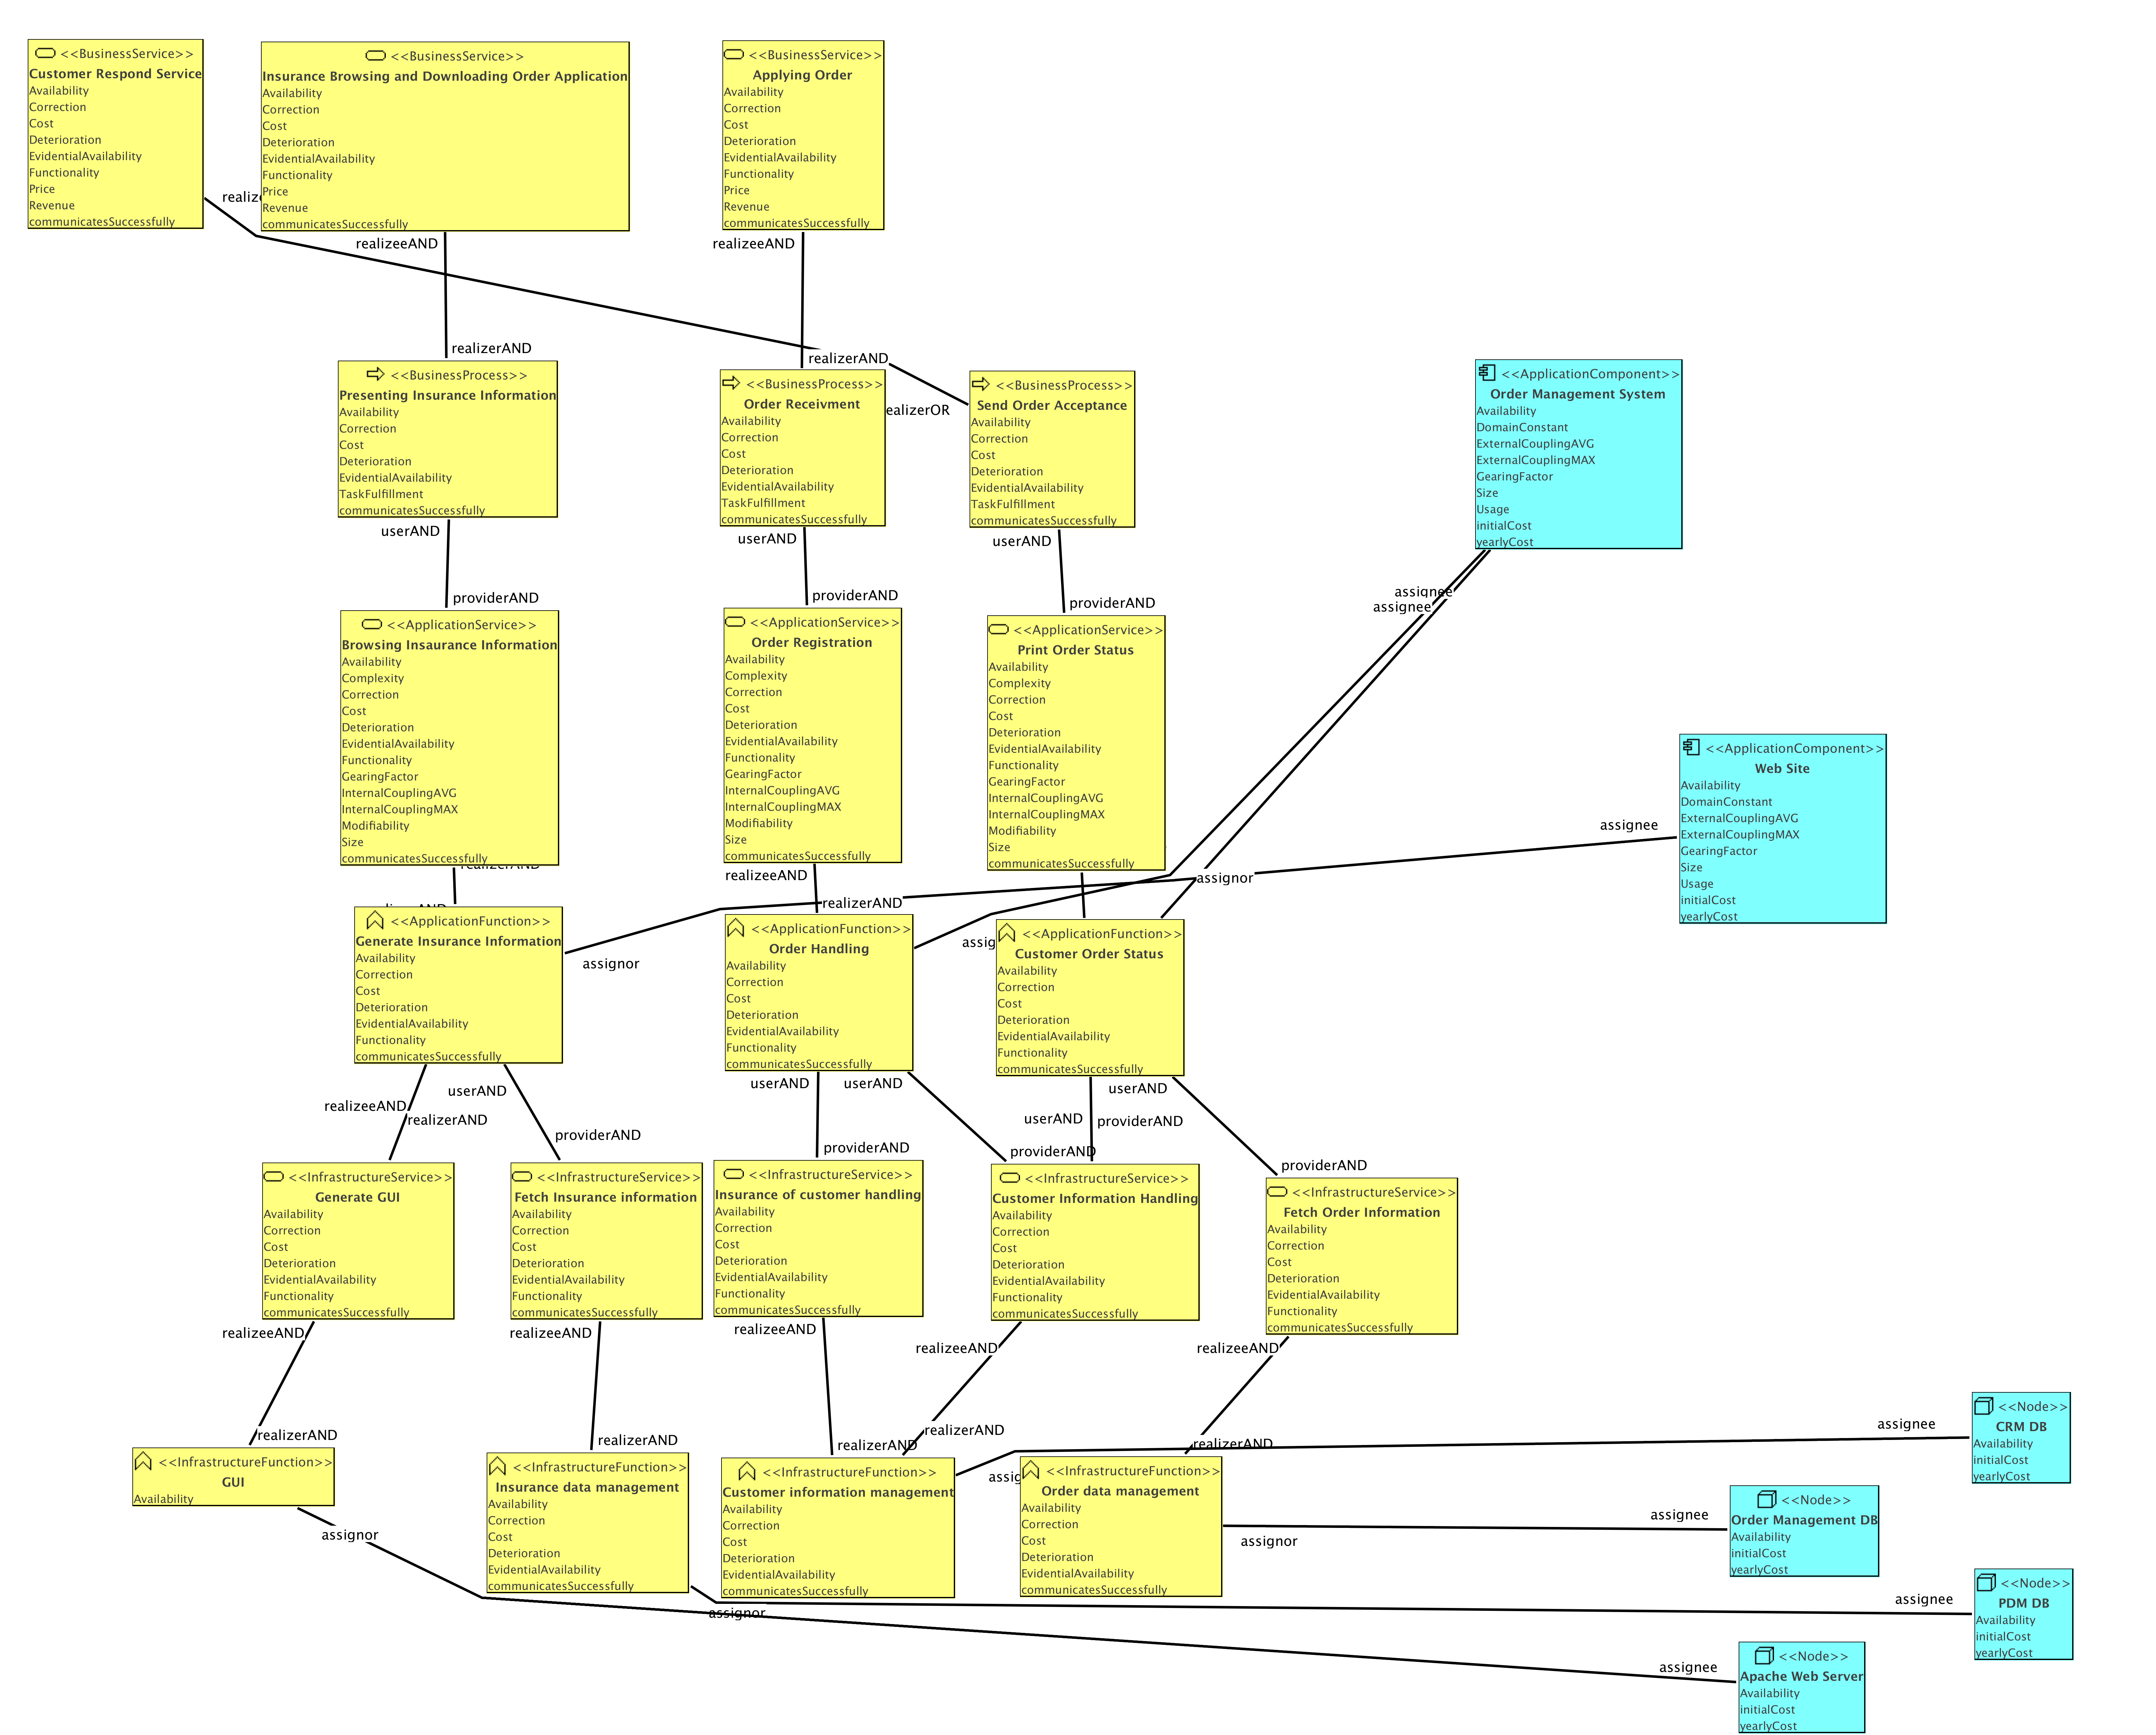
\includegraphics[scale = 0.05]{images/map_order_availability.png}}
		\caption{Cost of the processes "Order Receivement" and "Send Order Acceptance" (\emph{MAP})}
		\label{fig:map_order_availability}
	\end{figure}
\end{center}
Next we present the current values for some entities primarily considered when assessing the availability. The first two tables (Nodes \& Application components) are evidential values, meaning, that these are values already set and not computed with through the EAAT tool. Whereas the availability in table the last table are derived values by EAAT.
%
\subsection{Improvements}
\label{sec:improvements}
One could see improvements to the systems from the three analysis in the previous section. An improvement possible to increase the data accuracy in the analysis of the Claim registration is to create support on the website for claim registration, instead of having the customers to send an application to the company. This will then be represented the correct way directly from the system and the decrease of accuracy in the claim administrators work could be eliminated.\\\\
%
An improvement to the availability of the support services could be an aggregation of the two support services into one support service. An integrated more modern support system would be easier to maintain and the availability of the system would thereby increase.\\\\
%
An improvement to the cost of the order processing could also be to integrate the order processes into an automated system on the website, which then could eliminate the costs of the manager and as J.D.H. Insurance already has an web site, the costs for implementing it would not be very high and the cost for maintenance of that new functionality of the website would not be high since the website already is maintained. Hence, it would lower the costs.\\\\
%
Furthermore, the as-is model of the company illustrates the different collaboration between systems. For example, the CMS is currently interconnected with three other systems. CMS is and will be an important function in the enterprise and the results of improving it may be of great proportions if we find it deficient. If so, one key aspect we need to take into account when suggesting such a change is to study the application modifiability of the CMS. This will help us analyze the effects as well as the costs it may imply. Naturally, studying the modifiability will apply to every system, not just to the CMS.
\clearpage

\section{To-Be}
\label{sec:to_be}
This section will focus on the To-Be architecture of J.D.H. Insurance. Models and analysis of the target architecture will be presented, along with the gaps between the target architecture and the As-Is architecture. These gaps will be the foundation of the coming section.
%
\subsection{Models}
\label{sec:models}
In this section the models of the to-be architecture of J.D.H Insurance will be presented.
%
\subsection{Analysis}
\label{sec:analysis}
Analysis of the new architectural changes to the enterprise will be presented in this section.
%
\subsection{Comparison with as-is - Gaps}
\label{sec:gaps}
The gaps between the As-is model and the To-be model will be presented in this section.







\clearpage

\section{MAP Analysis}
\label{sec:map_analys}
\input{node_table.tex}
\begin{table}[H]
	\centering
	\begin{tabular}{|c|c|p{2cm}|p{2.5cm}|p{2.5cm}|p{2.5cm}|}
		\cline{3-6}

		\multicolumn{2}{c}{} & \multicolumn{4}{|c|}{\textbf{Nodes}} \\ \cline{3-6}
		\multicolumn{2}{c|}{} & \multicolumn{1}{c|}{\textsl{Phone System Dispatcher}} & \multicolumn{2}{c|}{\textsl{Mail DB}} & \multicolumn{1}{c|}{\textsl{Help Desk DB}}\\
		\hline
		\multirow{2}{*}{Availability} & As-Is & \multicolumn{1}{c|}{0.99} & \multicolumn{2}{c|}{0.98} & \multicolumn{1}{c|}{N/A}\\ \cline{2-6}
										& To-Be &\multicolumn{1}{c|}{-} & \multicolumn{2}{c|}{-} & \multicolumn{1}{c|}{HEAVY}\\ \hline

		\multicolumn{6}{c}{} \\ \cline{3-6}							
		\multicolumn{2}{c}{} & \multicolumn{4}{|c|}{\textbf{Application Components}} \\ \cline{3-6}
		\multicolumn{2}{c|}{} & \multicolumn{1}{c|}{\textsl{Phone Support System}} & \multicolumn{2}{c|}{\textsl{Mail Support System}} & \multicolumn{1}{c|}{\textsl{Help Desk System}}\\
		\hline
		\multirow{2}{*}{Availability} & As-Is & \multicolumn{1}{c|}{0.99} & \multicolumn{2}{c|}{0.99} & \multicolumn{1}{c|}{N/A}\\ \cline{2-6}
										& To-Be &\multicolumn{1}{c|}{N/A} & \multicolumn{2}{c|}{N/A} & \multicolumn{1}{c|}{0.98}\\ \hline

	   \multicolumn{6}{c}{} \\ \cline{3-6}
		\multicolumn{2}{c}{} & \multicolumn{4}{|c|}{\textbf{Role}} \\ \cline{3-6}
		\multicolumn{2}{c|}{} & \multicolumn{4}{|c|}{\textsl{Mail Supporter}}\\ \hline
		\multirow{2}{*}{Availability} & As-Is & \multicolumn{4}{|c|}{0.95}\\ \cline{2-6}
									   & To-Be & \multicolumn{4}{|c|}{-}\\ \hline

		\multicolumn{6}{c}{} \\ \cline{3-6}
		\multicolumn{2}{c}{} & \multicolumn{4}{|c|}{\textbf{Business Process}} \\ \cline{3-6}
		\multicolumn{2}{c|}{} & \multicolumn{4}{|c|}{\textsl{Send Response to Customer}}\\ \hline
		\multirow{2}{*}{Availability} & As-Is & \multicolumn{4}{|c|}{0.92}\\ \cline{2-6}
									   & To-Be & \multicolumn{4}{|c|}{-}\\ \hline
		\multicolumn{6}{c}{} \\ \cline{3-6}
		\multicolumn{2}{c}{} & \multicolumn{4}{|c|}{\textbf{Business Services}} \\ \cline{3-6}
		\multicolumn{2}{c|}{} & \multicolumn{2}{|c|}{\textsl{Call Phone Support Service}} & \multicolumn{2}{|c|}{\textsl{Send Mail to Support Service}}\\ \hline
		\multirow{2}{*}{Availability} & As-Is & \multicolumn{2}{|c|}{0.91} & \multicolumn{2}{|c|}{0.94}\\ \cline{2-6}
									   & To-Be & \multicolumn{2}{|c|}{-} & \multicolumn{2}{|c|}{-}\\ \hline
	\end{tabular}
\caption{Support availability}
\label{tab:data_accuracy}
\end{table}
\begin{table}[H]
	\centering
	\begin{tabular}{|c|c|p{2cm}|p{2.5cm}|p{2.5cm}|p{2.5cm}|}
		\cline{3-6}

		\multicolumn{2}{c}{} & \multicolumn{4}{|c|}{\textbf{Nodes}} \\ \cline{3-6}
		\multicolumn{2}{c|}{} & \multicolumn{1}{c|}{\textsl{Apache Web Server}} & \multicolumn{1}{c|}{\textsl{PDM DB}} & \multicolumn{1}{c|}{\textsl{CRM DB}} & \multicolumn{1}{c|}{\textsl{Order Management DB}}\\
		\hline
		\multirow{2}{*}{Availability} & As-Is & \multicolumn{1}{c|}{0.99} & \multicolumn{1}{c|}{0.99} & \multicolumn{1}{c|}{0.97} & \multicolumn{1}{c|}{0.98}\\ \cline{2-6}
										& To-Be &\multicolumn{1}{c|}{-} & \multicolumn{2}{c|}{-} & \multicolumn{1}{c|}{-}\\ \hline

		\multicolumn{6}{c}{} \\ \cline{3-6}							
		\multicolumn{2}{c}{} & \multicolumn{4}{|c|}{\textbf{Application Components}} \\ \cline{3-6}
		\multicolumn{2}{c|}{} & \multicolumn{2}{c|}{\textsl{Order Management System}} & \multicolumn{2}{c|}{\textsl{Web Site}}\\
		\hline
		\multirow{2}{*}{Availability} & As-Is & \multicolumn{2}{c|}{0.99} & \multicolumn{2}{c|}{0.99}\\ \cline{2-6}
										& To-Be &\multicolumn{2}{c|}{-} & \multicolumn{2}{c|}{-}\\ \hline

		\multicolumn{6}{c}{} \\ \cline{3-6}
		\multicolumn{2}{c}{} & \multicolumn{4}{|c|}{\textbf{Business Process}} \\ \cline{3-6}
		\multicolumn{2}{c|}{} & \multicolumn{4}{|c|}{\textsl{Send Order Acceptance}}\\ \hline
		\multirow{2}{*}{Availability} & As-Is & \multicolumn{4}{|c|}{0.89}\\ \cline{2-6}
									   & To-Be & \multicolumn{4}{|c|}{-}\\ \hline
		\multicolumn{6}{c}{} \\ \cline{3-6}
		\multicolumn{2}{c}{} & \multicolumn{4}{|c|}{\textbf{Business Services}} \\ \cline{3-6}

		\multicolumn{2}{c|}{} & \multicolumn{2}{|p{5cm}|}{\textsl{Insurance Browsing and Downloading Order Application}} & \multicolumn{2}{|c|}{\textsl{Applying Order}} \\ \hline
		\multirow{2}{*}{Availability} & As-Is & \multicolumn{2}{|c|}{0.98} & \multicolumn{2}{|c|}{0.88}\\ \cline{2-6}
									   & To-Be & \multicolumn{2}{|c|}{-} & \multicolumn{2}{|c|}{-}\\ \hline
	\end{tabular}
\caption{Order availability}
\label{tab:data_accuracy}
\end{table}



\clearpage

\section{Transformation Plan}
\label{sec:transformation_plan}
The transformation plan from the As-is architecture to the To-be architecture will be presented during this section and will be based on the gaps found in the previous section.
\clearpage

\addcontentsline{toc}{section}{References}
\begin{thebibliography}{99}     
	
%\bibitem{gott2} \emph{Gottesdiener, Ellen. \textsl{"The Software Requirements Memmory Jogger" chapter 2}. GOAL/QPC, 2005}

\bibitem{idi.ntnu} \emph{Eide, Petter L. H. \textsl{''Quantification and Traceability of Requirements''} Gathered 2012-12-09 } <\url{http://www.idi.ntnu.no/grupper/su/fordypningsprosjekt-2005/eide-fordyp05.pdf}>

% \bibitem{projectsmart} \emph{Singh, Manjeet. \textsl{"Rescuing Projects in Crisis: Project Turnaround Pointers"} Gathered 2012-11-20} <\url{http://www.projectsmart.co.uk/rescuing-projects-in-crisis.html}> 

\bibitem{A} \emph{The ACME Power Company: Appendix A}

\bibitem{B} \emph{Work Order Management Systems Basics: Appendix B}

%\bibitem{I} \emph{Project plan for procurement project: Assignment I}

\bibitem{coleyconsulting} \emph{\textsl{"MoSCoW Prioritisation"} Gathered 2012-12-02} <\url{http://www.coleyconsulting.co.uk/moscow.htm}>

\bibitem{bpmn} Stephen A. White. \textsl{Introduction to BPMN Gathered 2012-12-04} <\url{https://bilda.kth.se/courseId/9302/node.do?id=19821584&ts=1350028814721&u=-1455921741}> 

\end{thebibliography}
\clearpage

\appendix
\section{As-Is MAP Models}
\label{sec:as_is_map_model}
\subsection{Business Architecture}
\begin{center}
	\begin{figure}[H]
		\centering
		\setlength\fboxsep{7pt}
		\setlength\fboxrule{0.5pt}
		\fbox{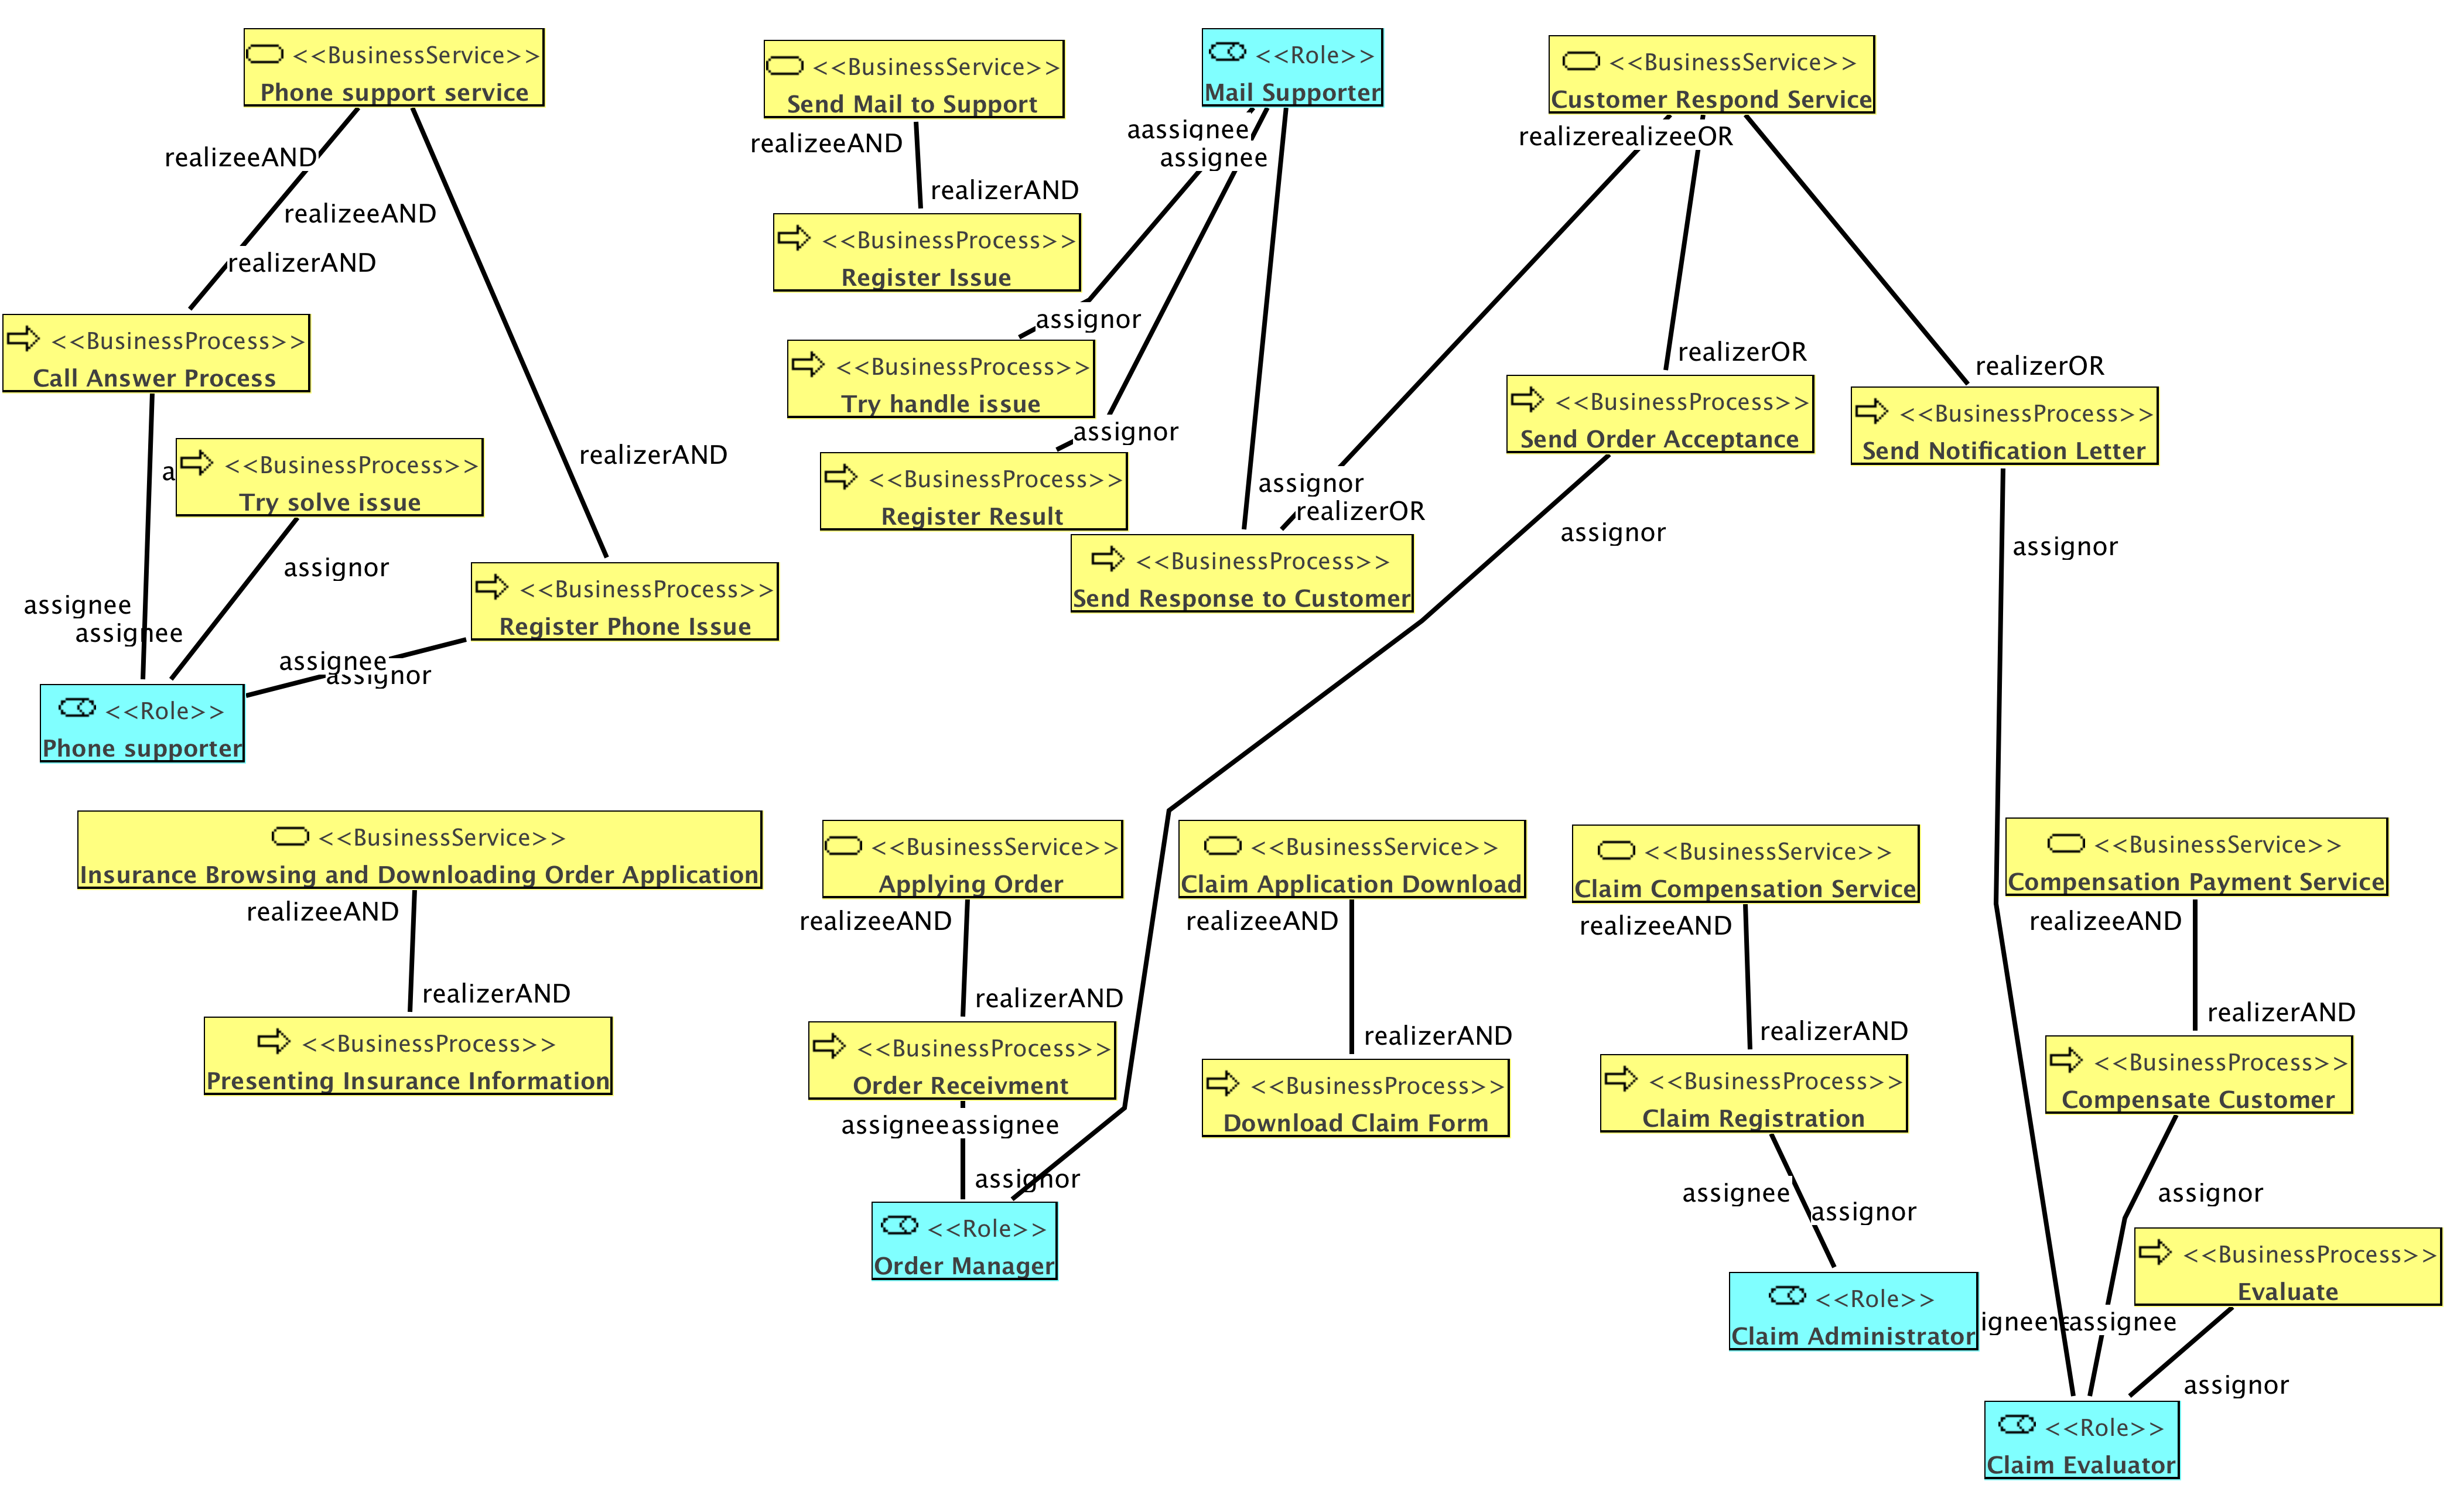
\includegraphics[scale = 0.14, angle=90]{images/map_business_asis.png}}
		\caption{As-Is Business Architecture}
		\label{fig:map_business_as_is}
	\end{figure}
\end{center}
%
\vspace{-5cm}
\subsection{Information Architecture}
\begin{center}
	\begin{figure}[H]
		\centering
		\setlength\fboxsep{7pt}
		\setlength\fboxrule{0.5pt}
		\fbox{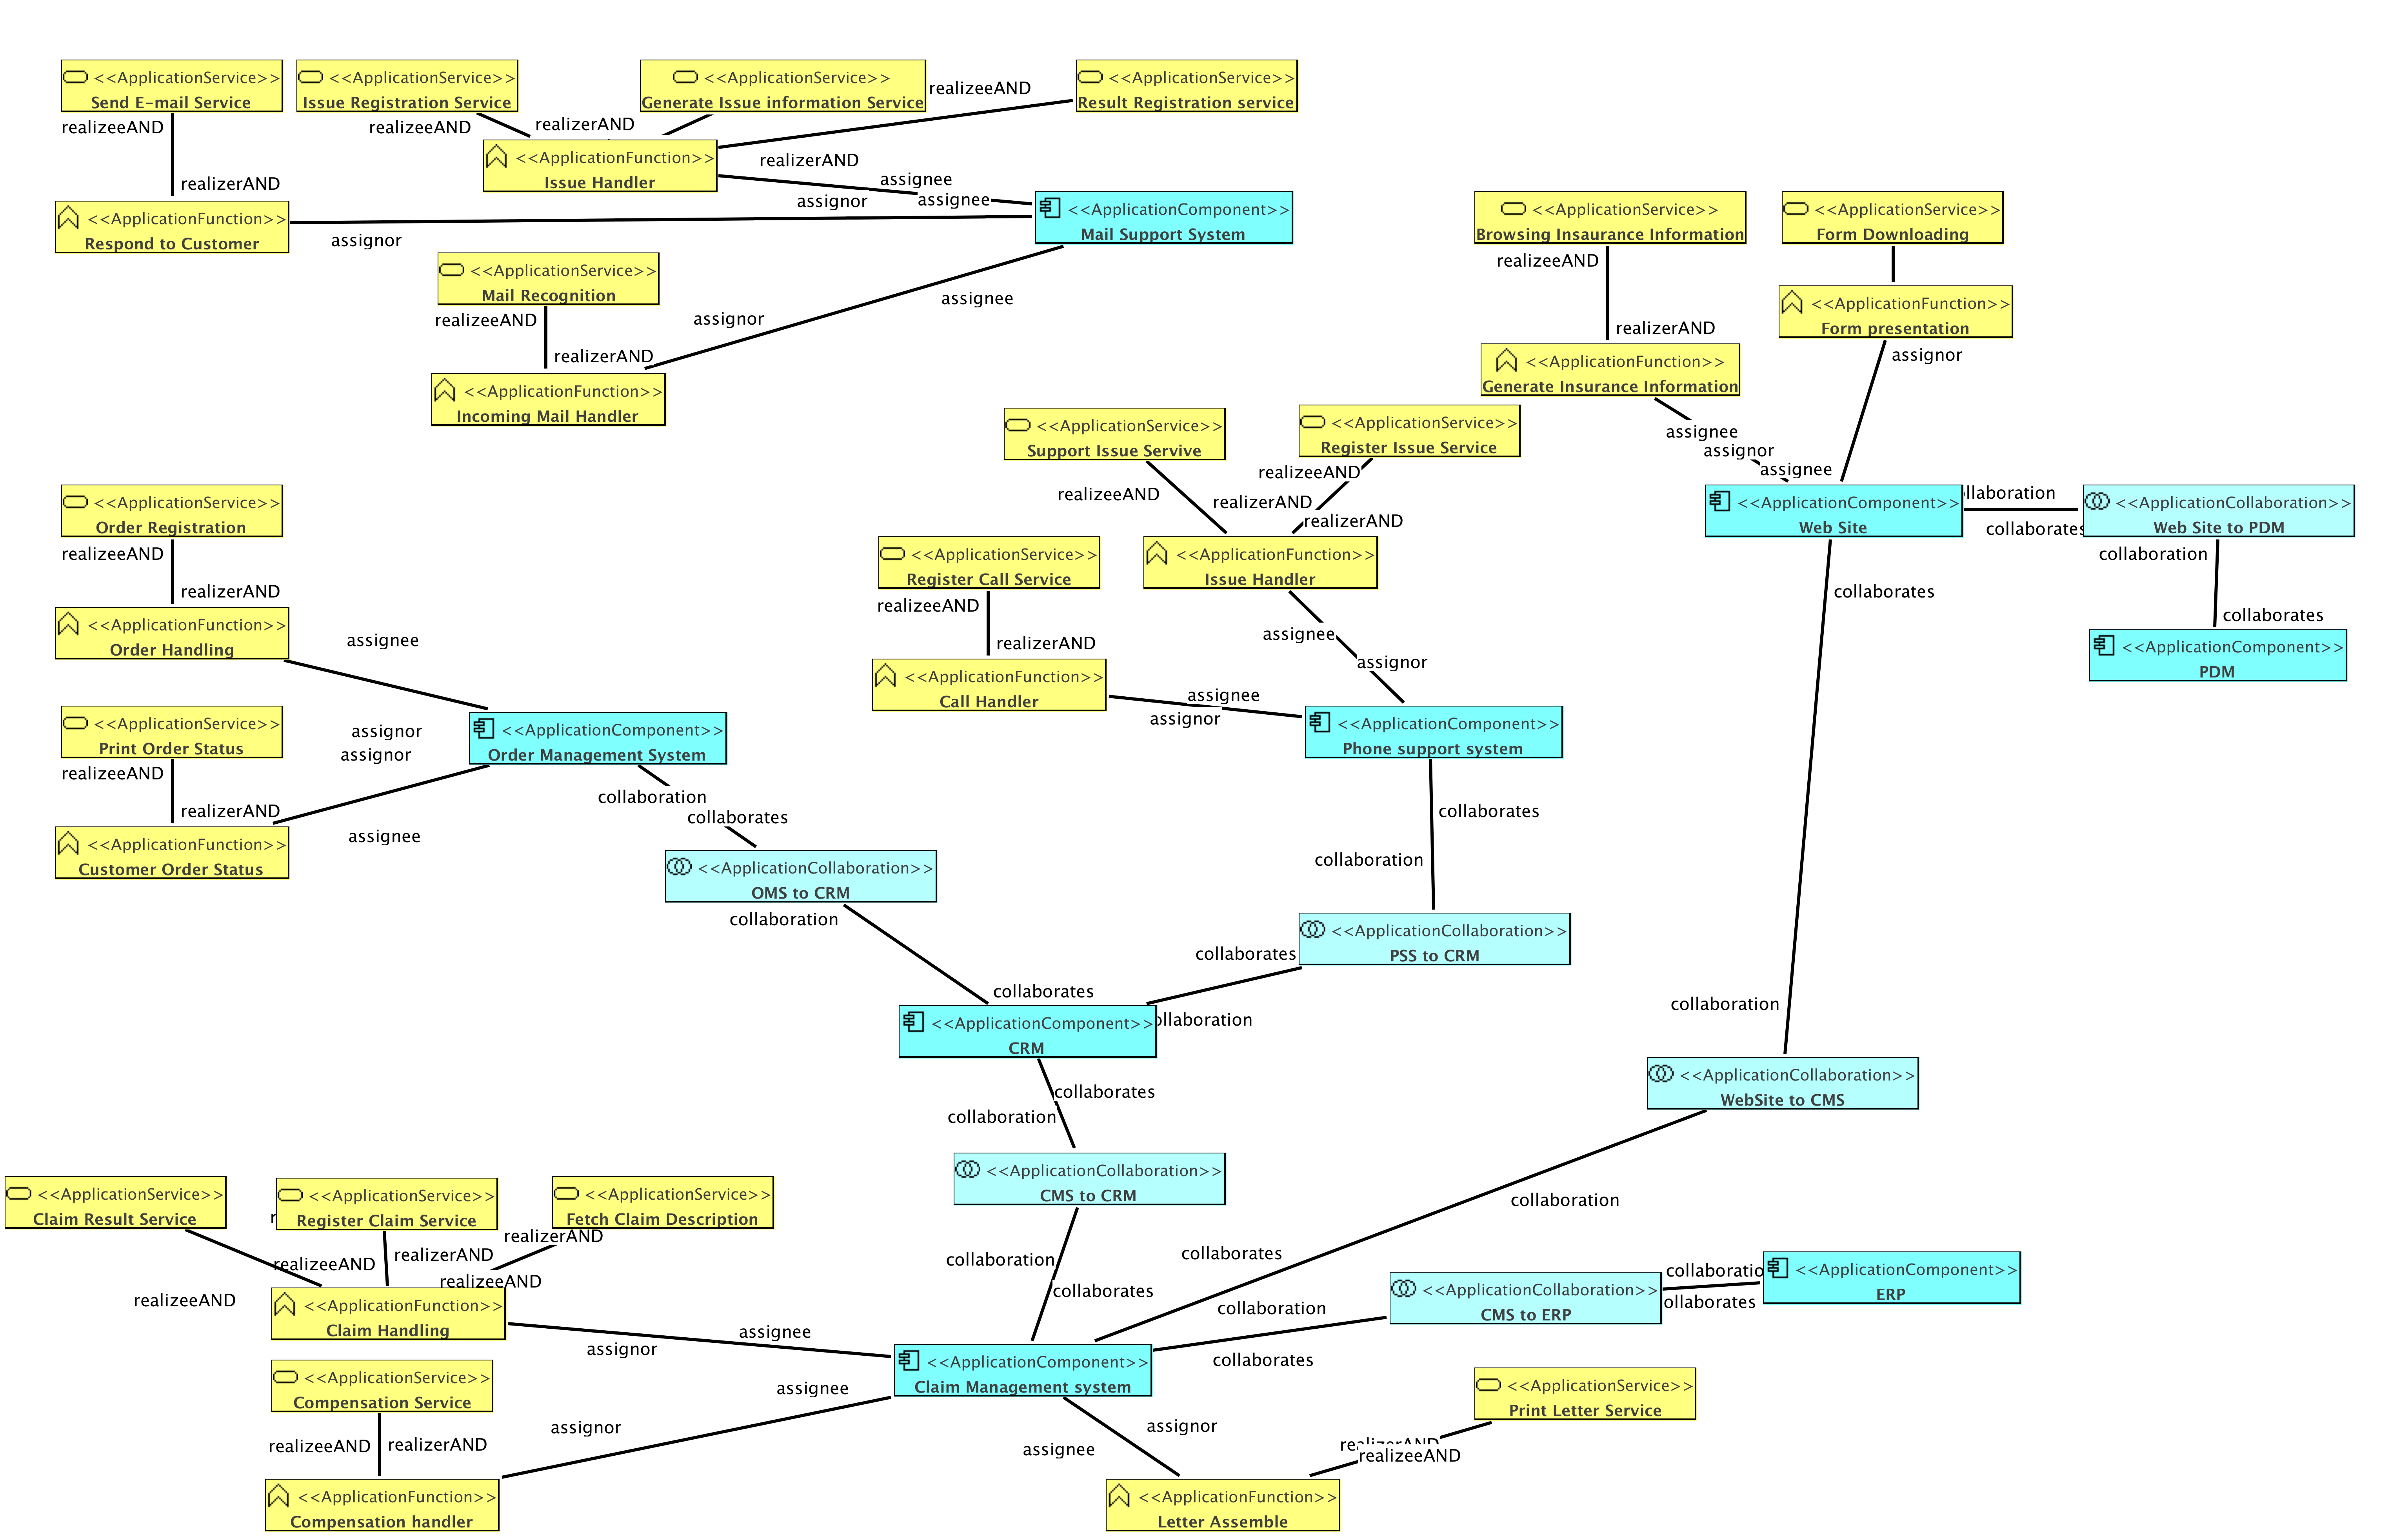
\includegraphics[scale = 0.09, angle=90]{images/map_application_asis.png}}
		\caption{As-Is Information Architecture}
		\label{fig:map_application_as_is}
	\end{figure}
\end{center}
%
\subsection{Information System Architecture}
\begin{center}
	\begin{figure}[H]
		\centering
		\setlength\fboxsep{7pt}
		\setlength\fboxrule{0.5pt}
		\fbox{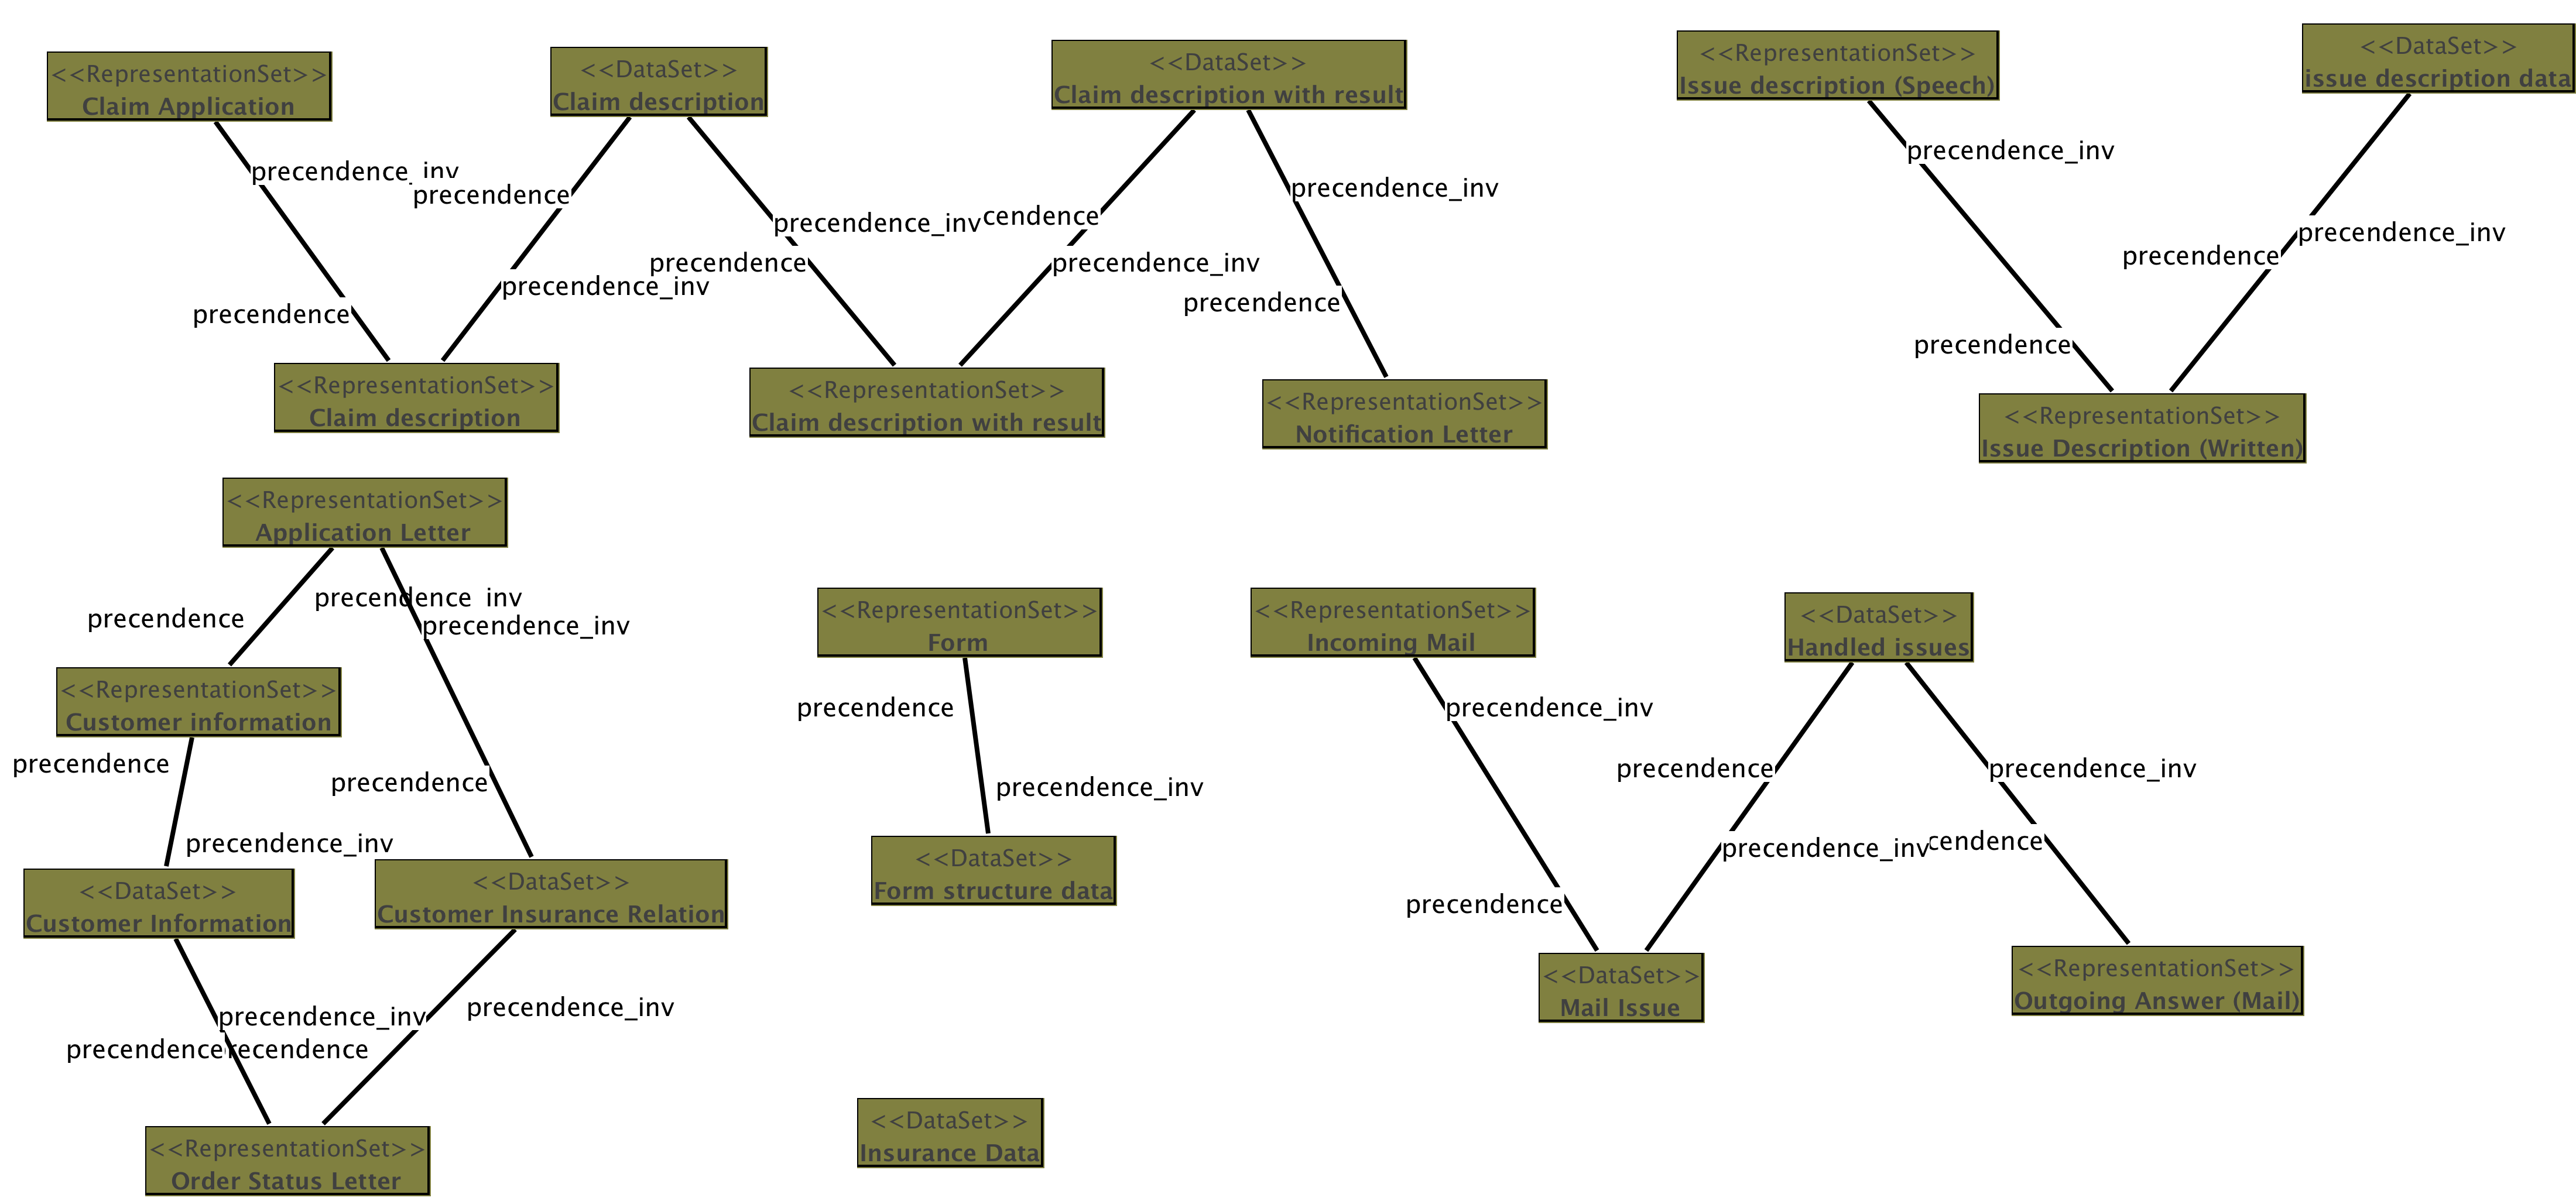
\includegraphics[scale = 0.13, angle=90]{images/map_information_asis.png}}
		\caption{As-Is Information System Architecture}
		\label{fig:map_information_as_is}
	\end{figure}
\end{center}
%
\subsection{Infrastructure Architecture}
\begin{center}
	\begin{figure}[H]
		\centering
		\setlength\fboxsep{7pt}
		\setlength\fboxrule{0.5pt}
		\fbox{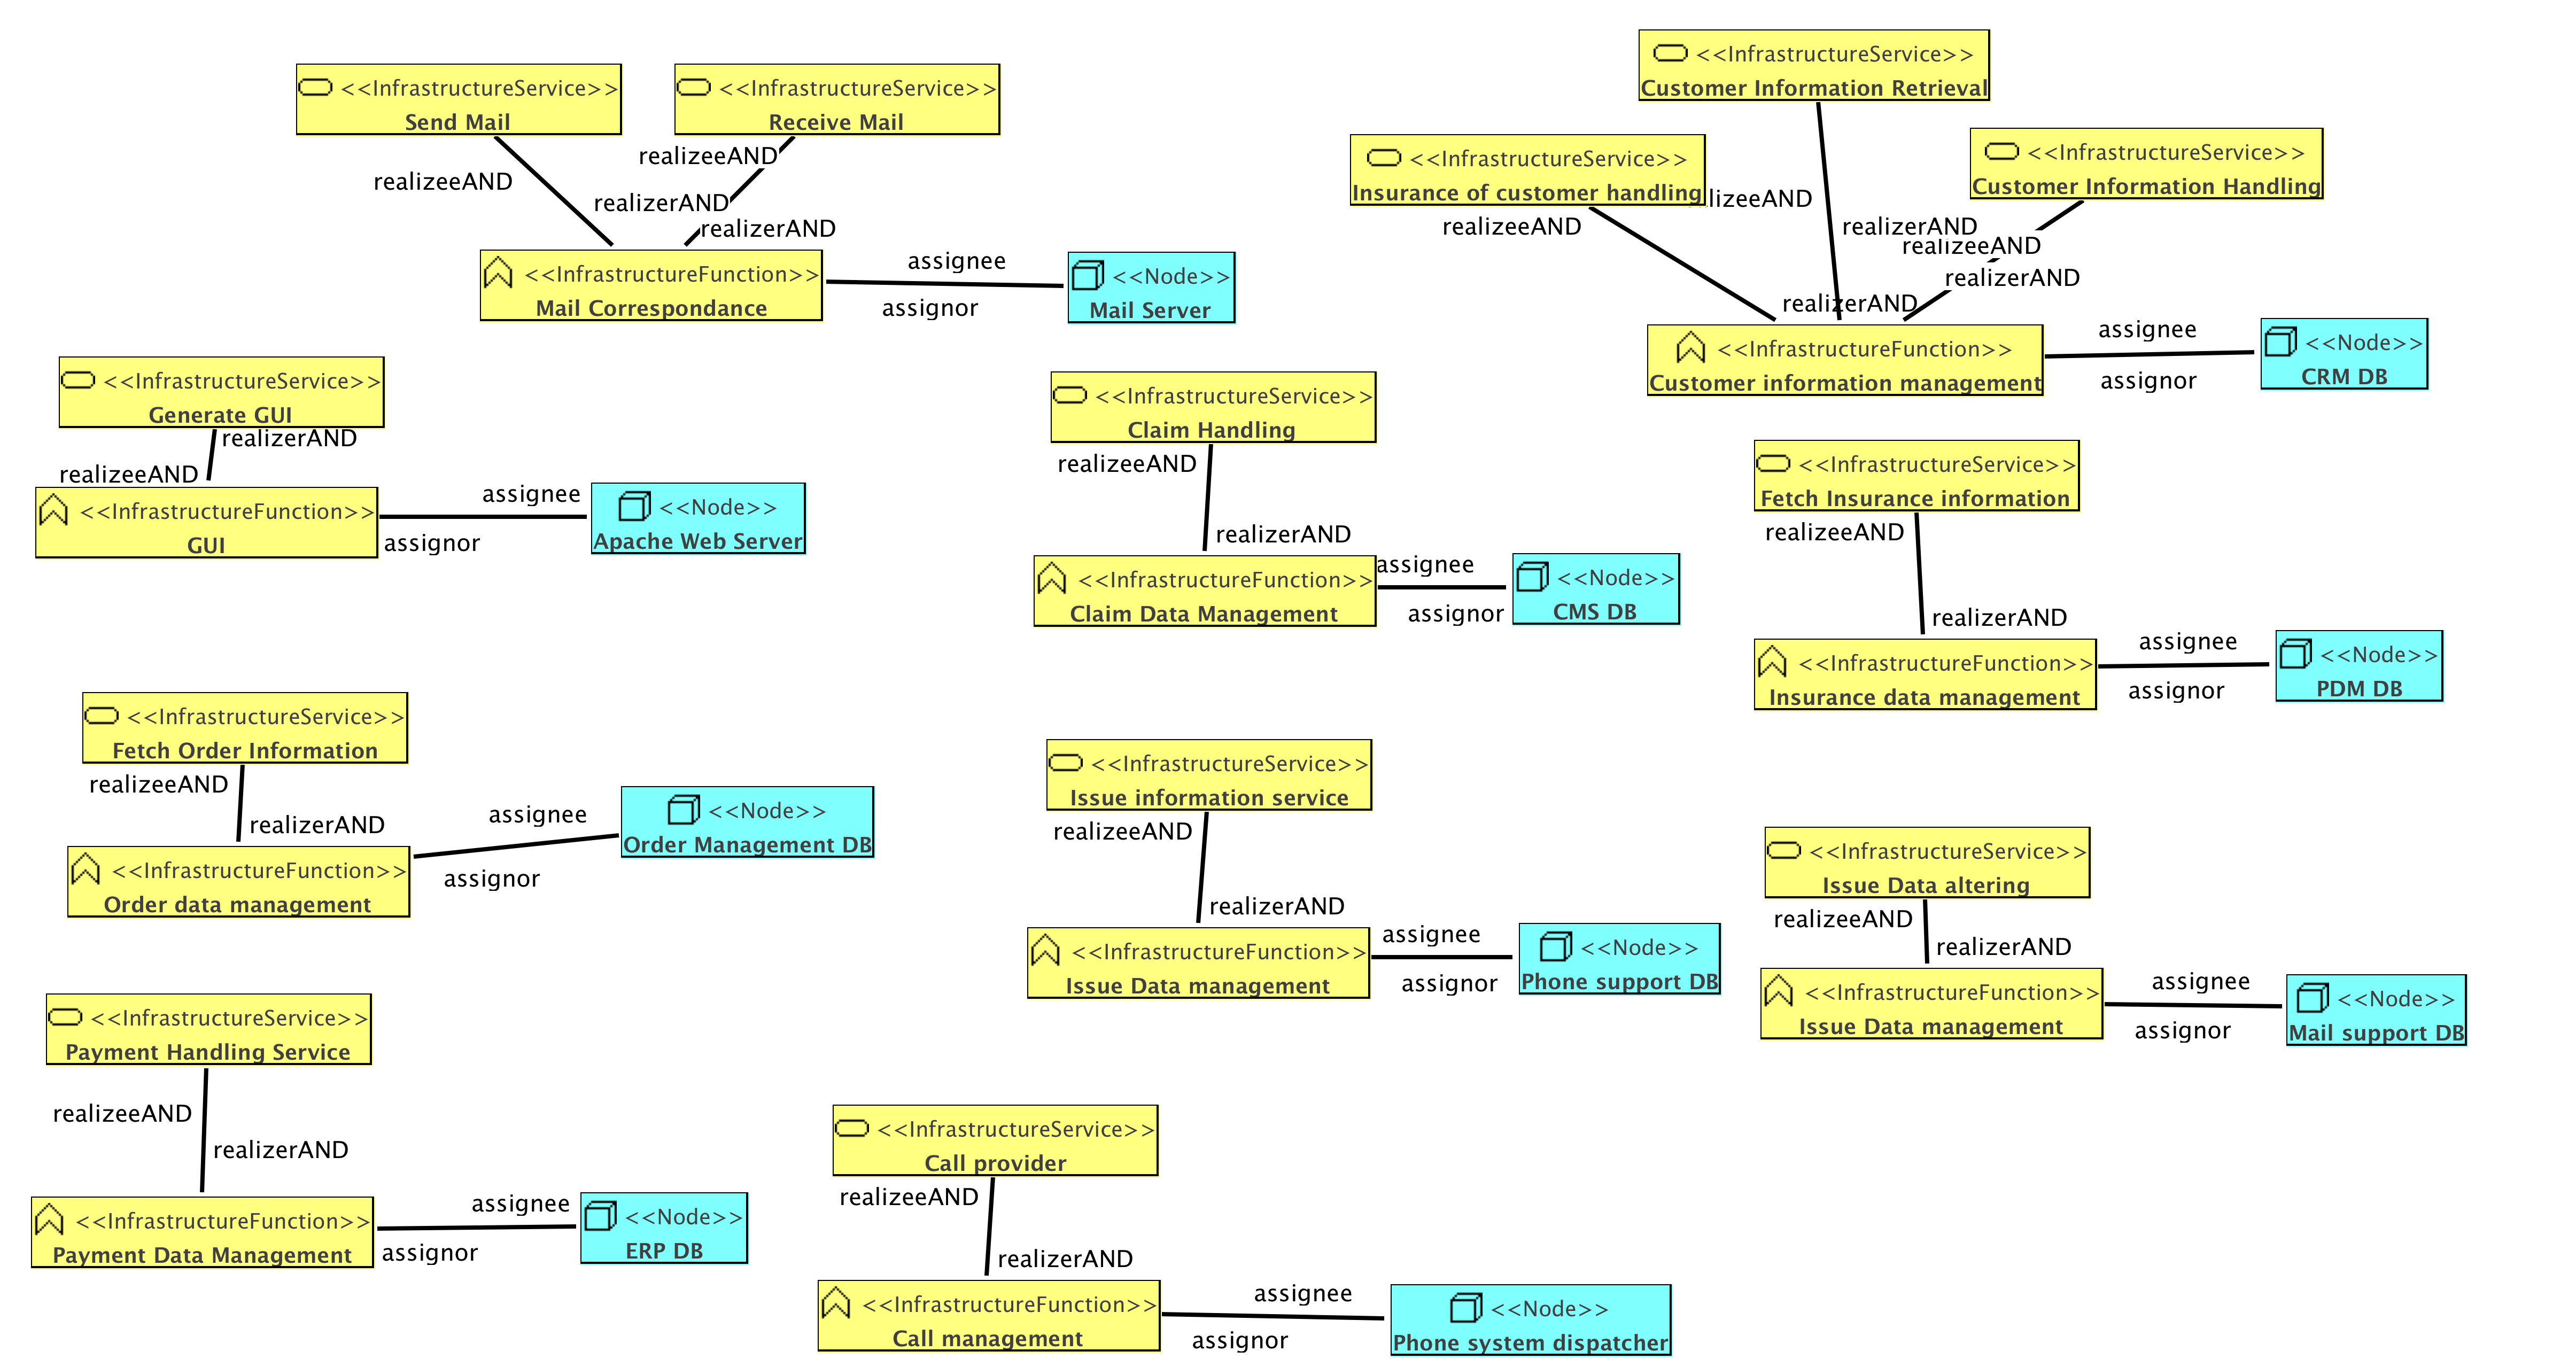
\includegraphics[scale = 0.12, angle=90]{images/map_infrastructure_asis.png}}
		\caption{As-Is Infrastructre Architecture}
		\label{fig:map_information_as_is}
	\end{figure}
\end{center}

\section{To-Be MAP Models}
\label{sec:to_be_map_model}
\subsection{Business Architecture}
\begin{center}
	\begin{figure}[H]
		\centering
		\setlength\fboxsep{7pt}
		\setlength\fboxrule{0.5pt}
		%\fbox{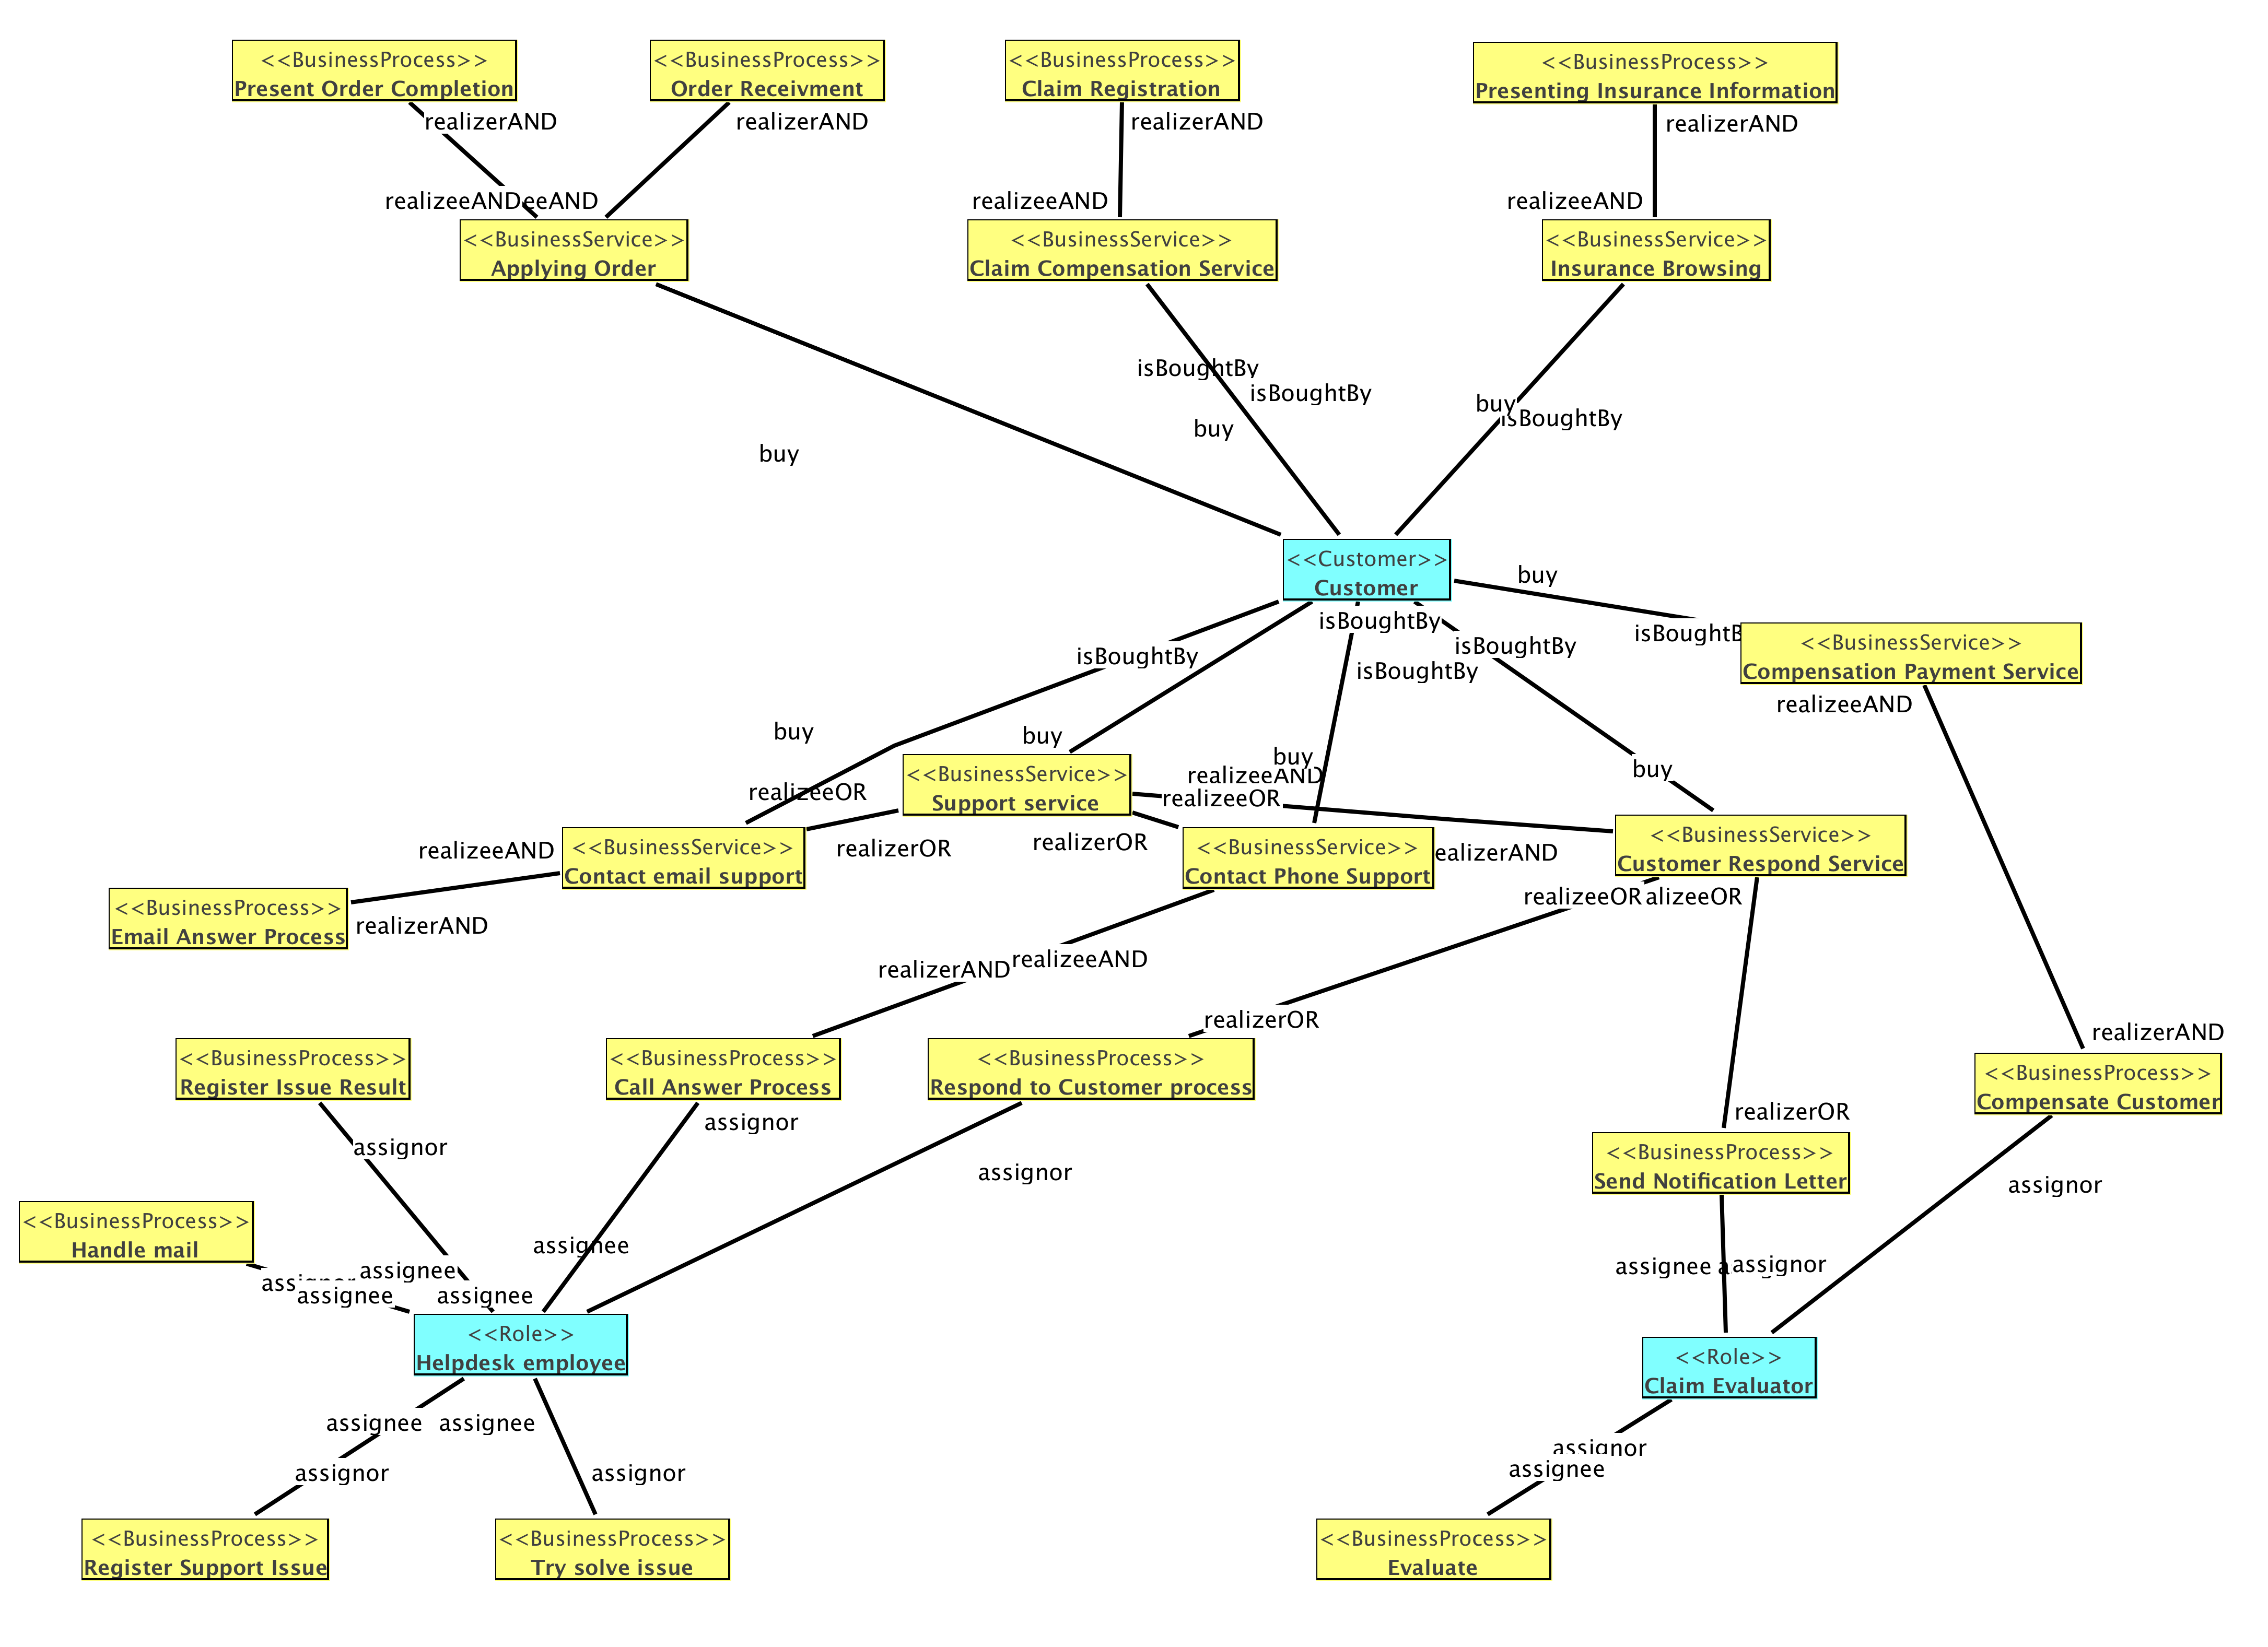
\includegraphics[scale = 0.14, angle=90]{images/map_business_tobe.png}}
		\caption{To-Be Business Architecture}
		\label{fig:map_business_to_be}
	\end{figure}
\end{center}
%
\vspace{-5cm}
\subsection{Information Architecture}
\begin{center}
	\begin{figure}[H]
		\centering
		\setlength\fboxsep{7pt}
		\setlength\fboxrule{0.5pt}
		%\fbox{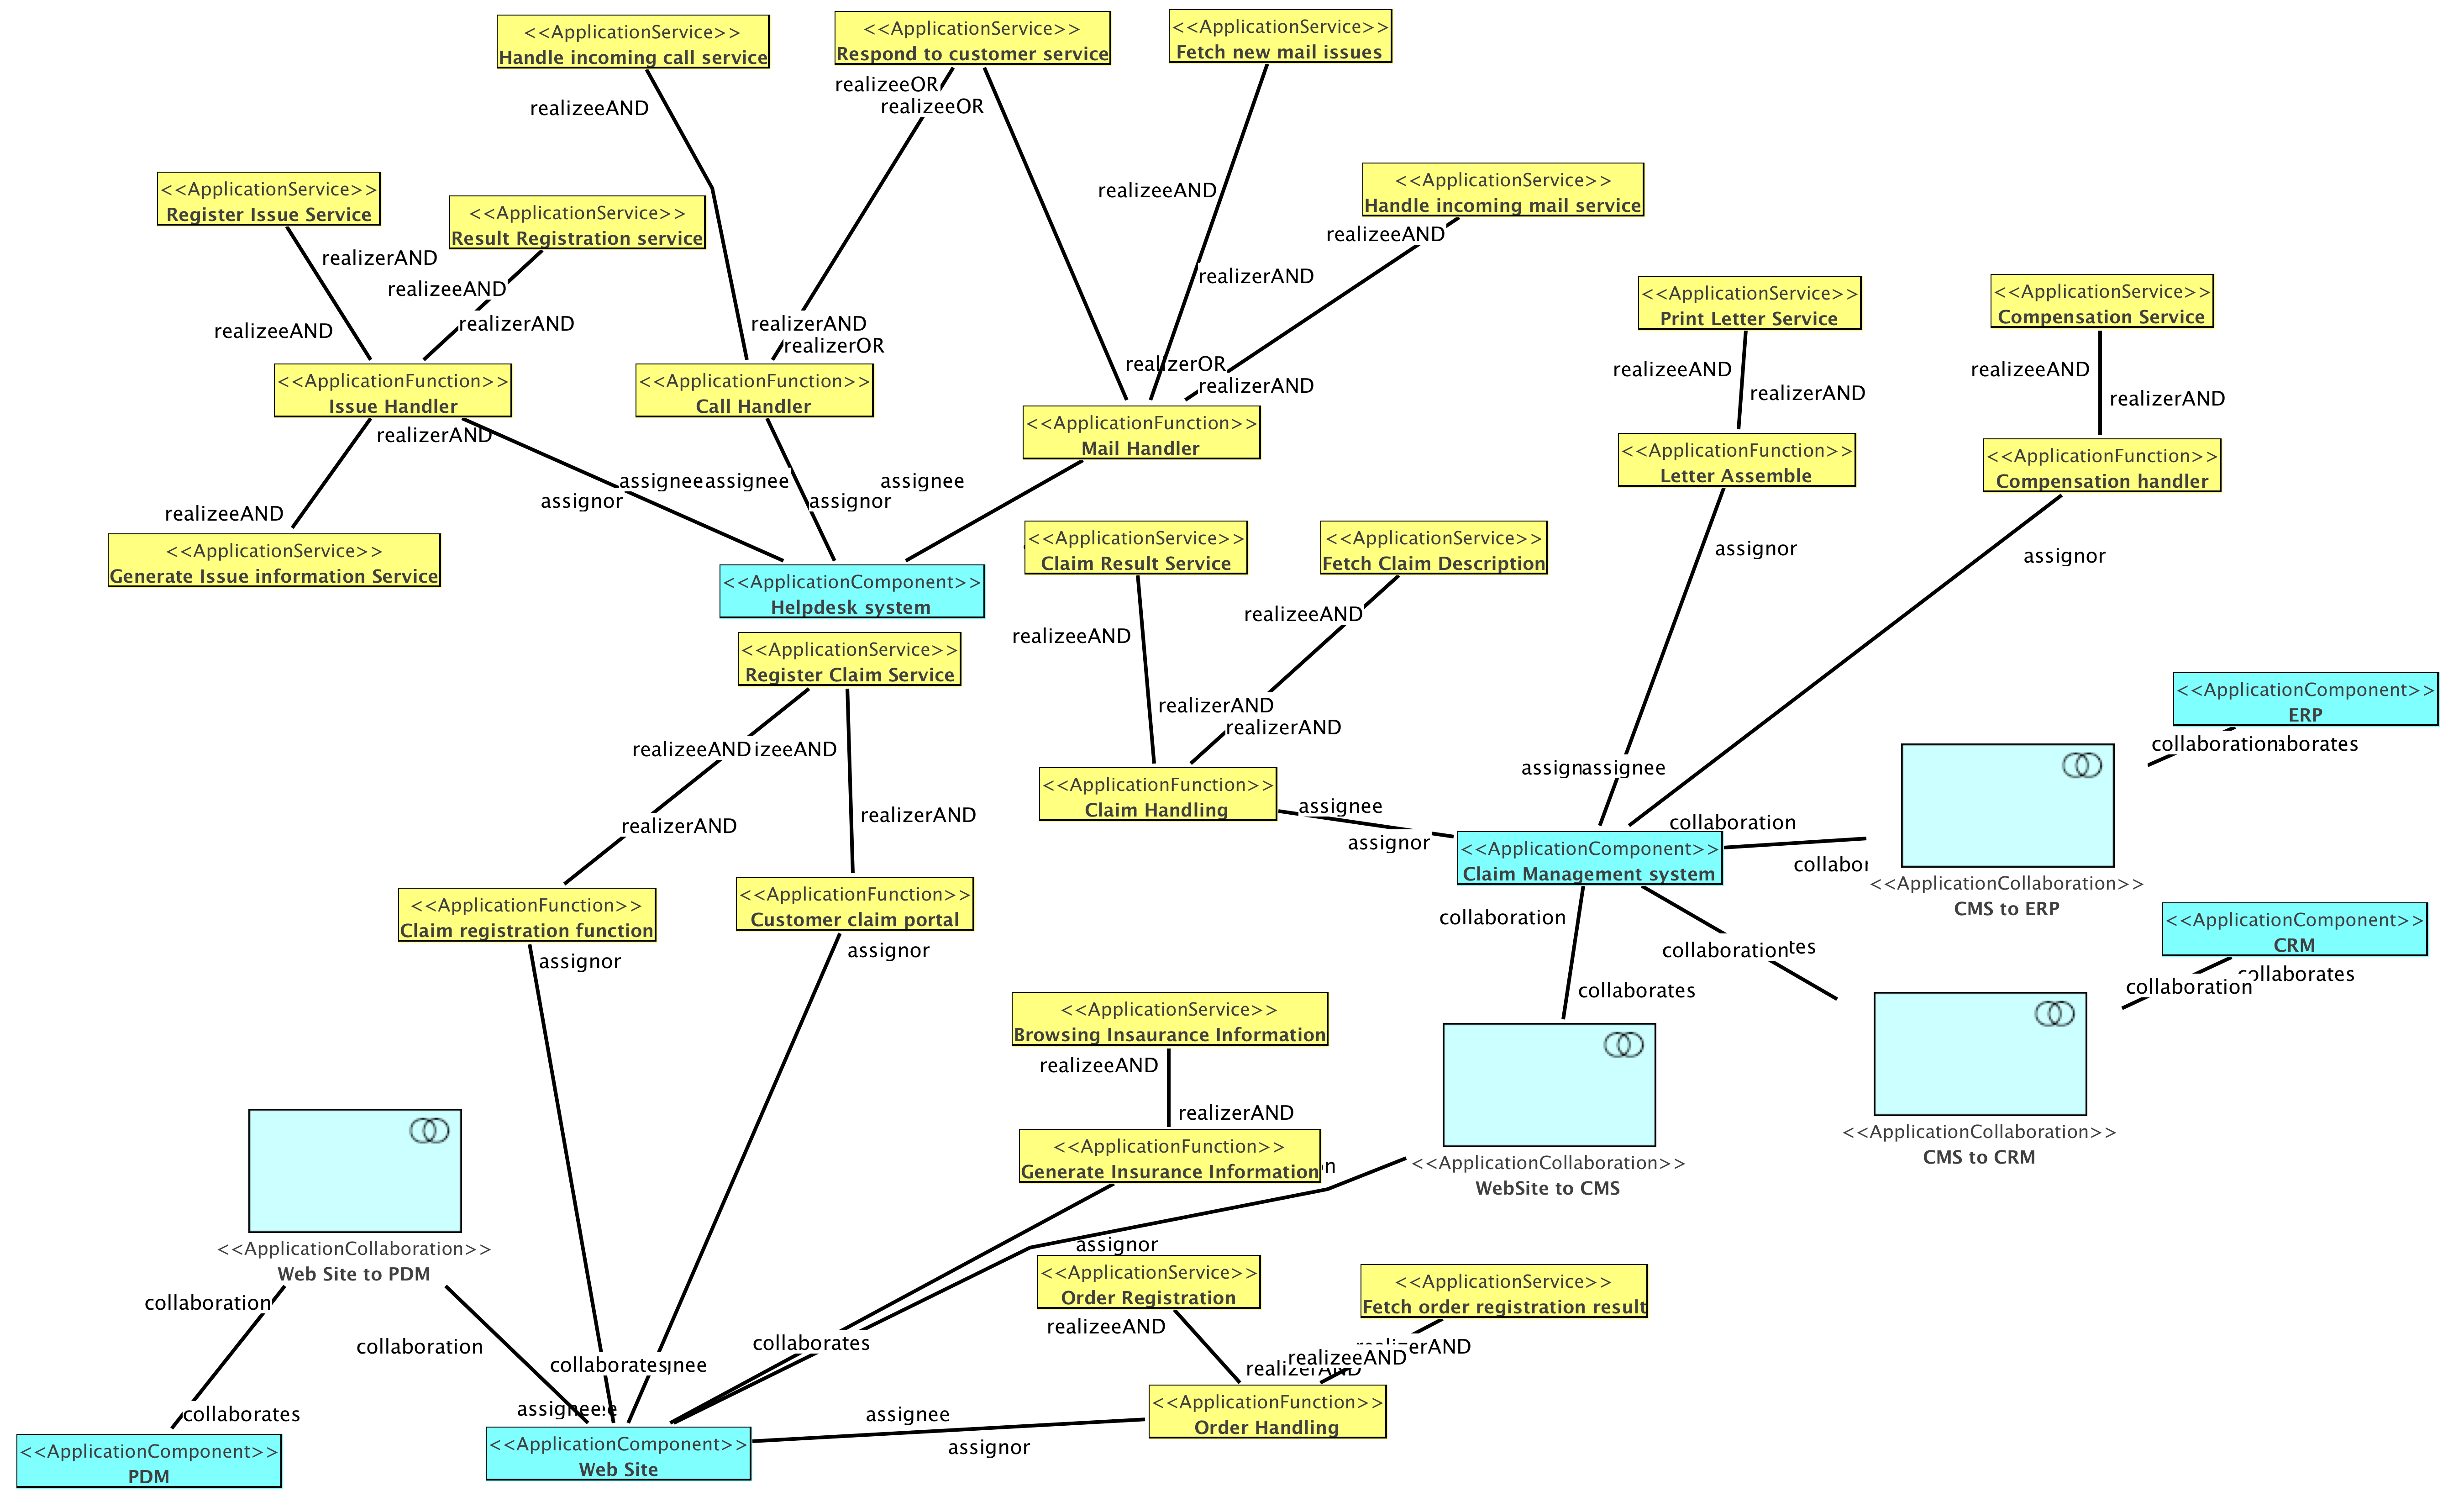
\includegraphics[scale = 0.09, angle=90]{images/map_application_tobe.png}}
		\caption{To-Be Information Architecture}
		\label{fig:map_application_to_be}
	\end{figure}
\end{center}
%
\subsection{Information System Architecture}
\begin{center}
	\begin{figure}[H]
		\centering
		\setlength\fboxsep{7pt}
		\setlength\fboxrule{0.5pt}
		%\fbox{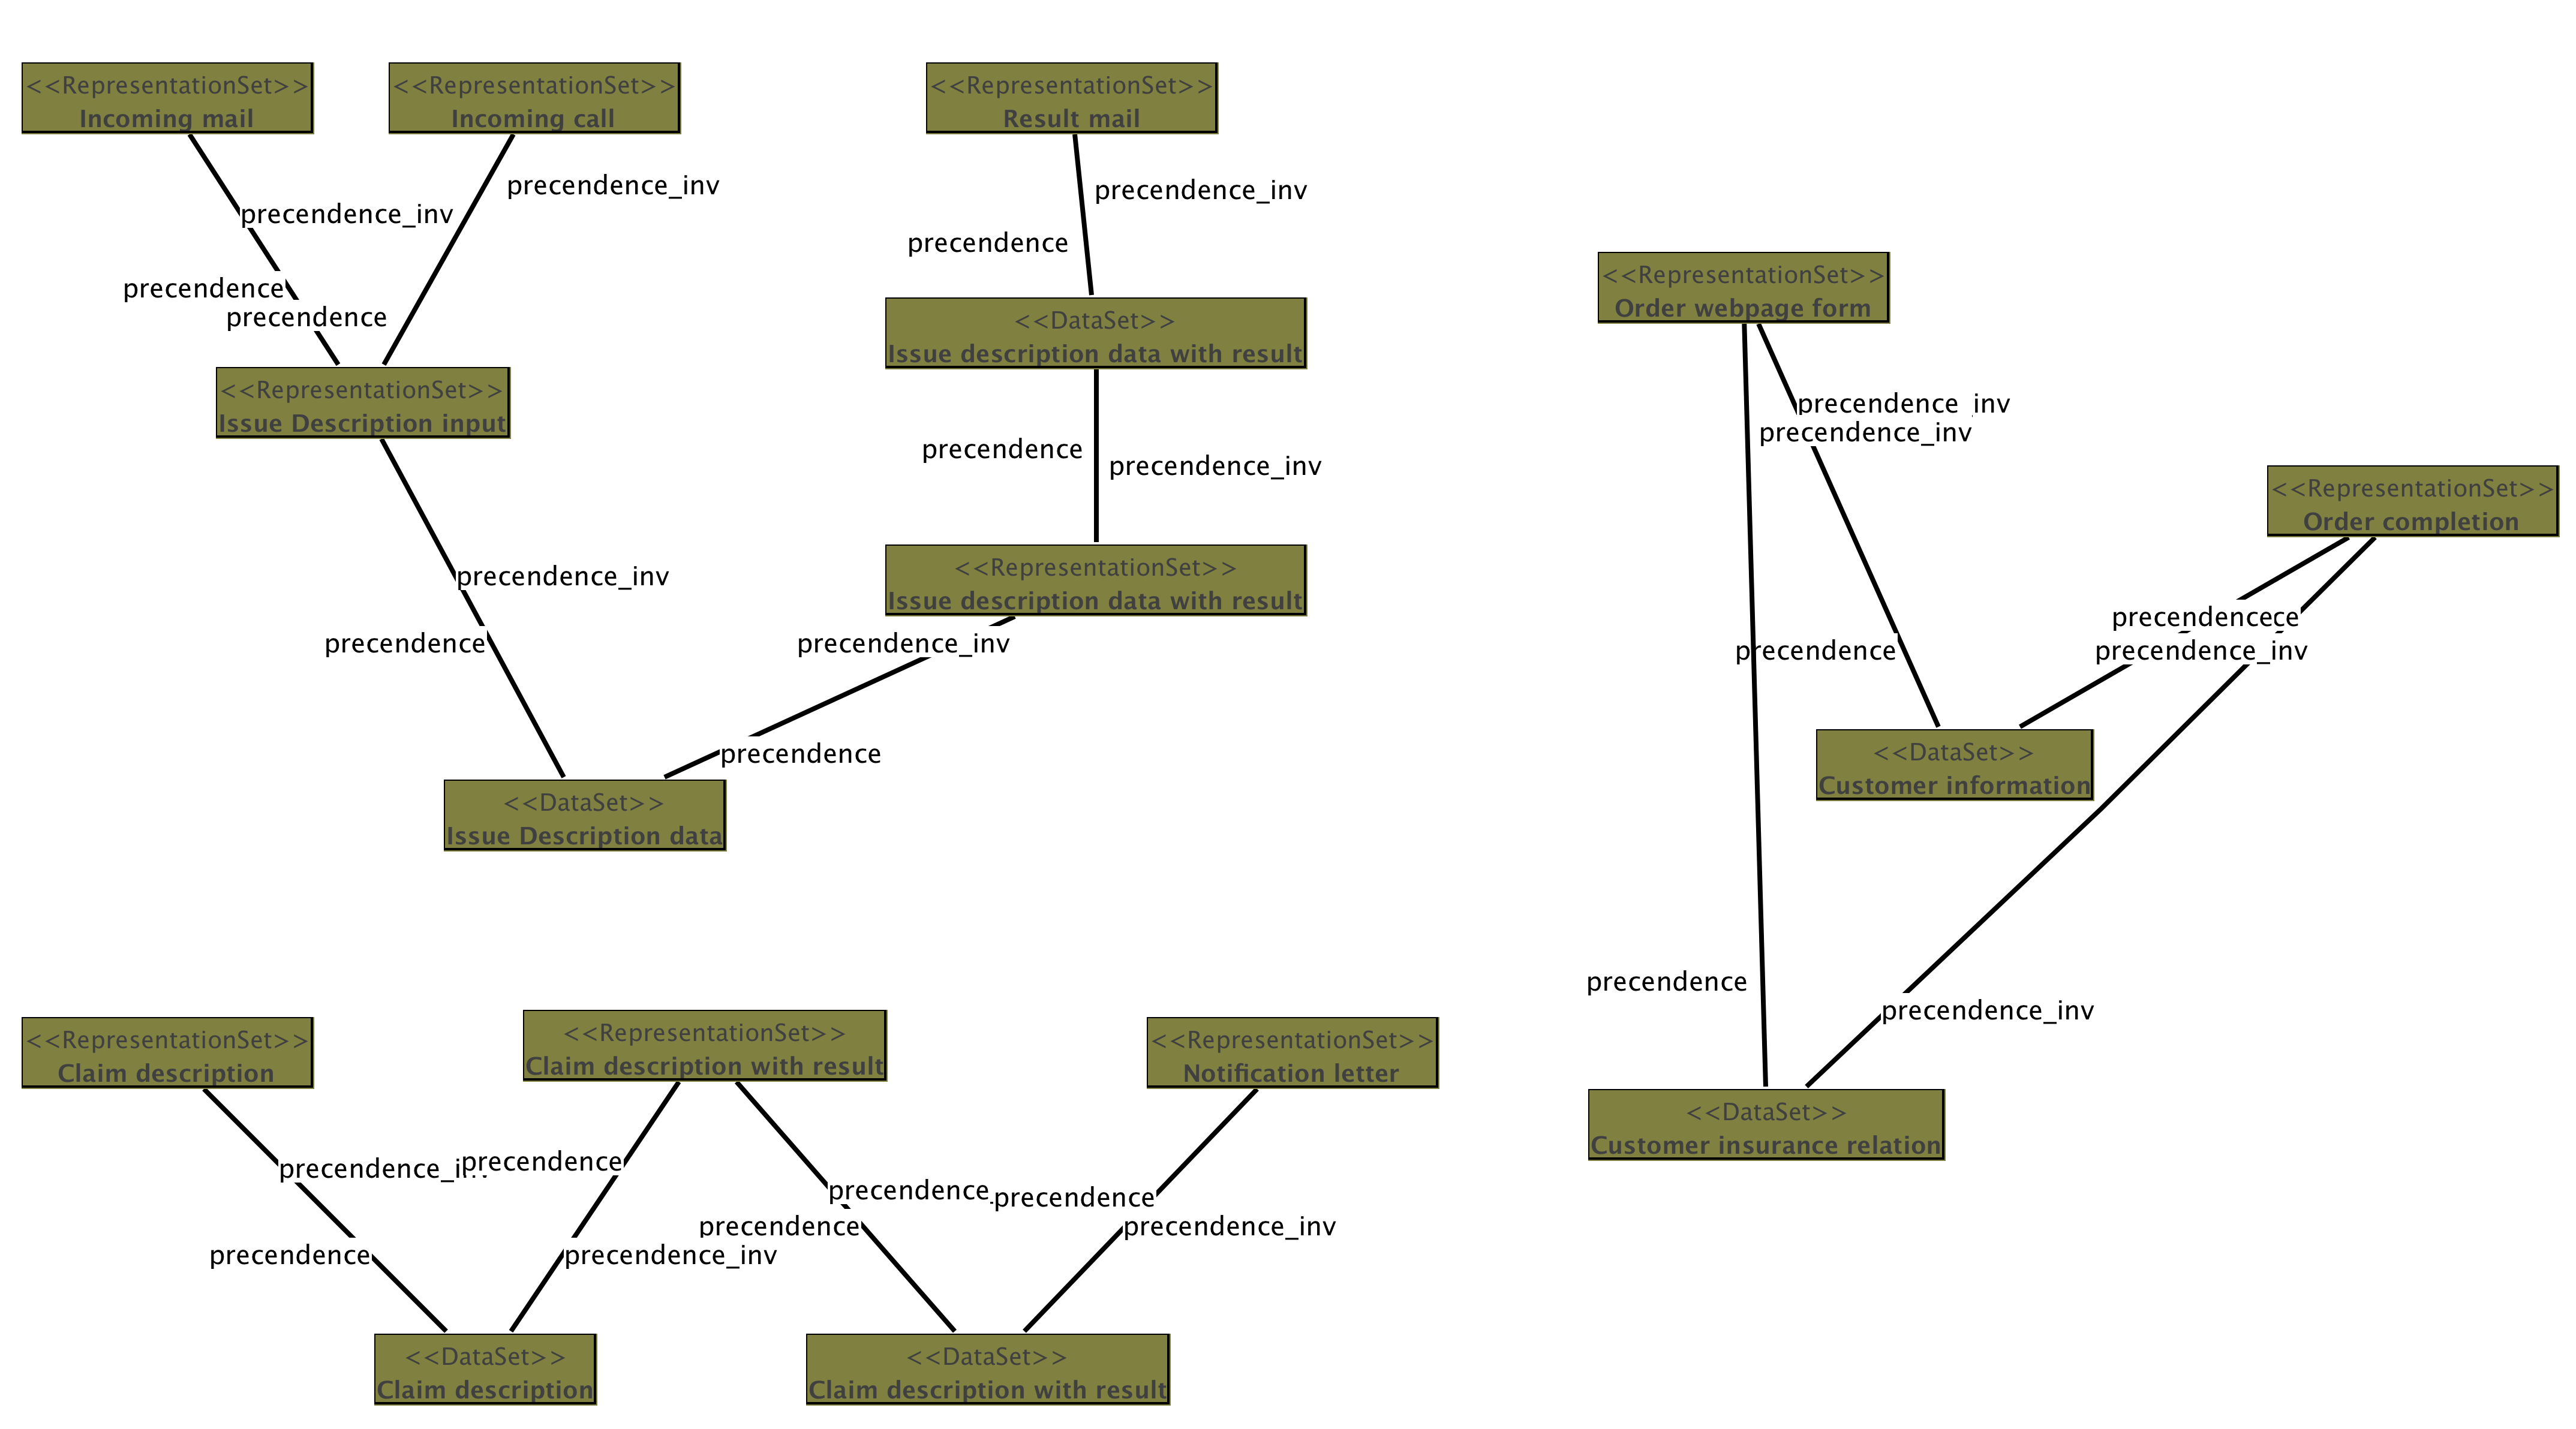
\includegraphics[scale = 0.13, angle=90]{images/map_information_tobe.png}}
		\caption{To-Be Information System Architecture}
		\label{fig:map_information_to_be}
	\end{figure}
\end{center}
%
\subsection{Infrastructure Architecture}
\begin{center}
	\begin{figure}[H]
		\centering
		\setlength\fboxsep{7pt}
		\setlength\fboxrule{0.5pt}
		%\fbox{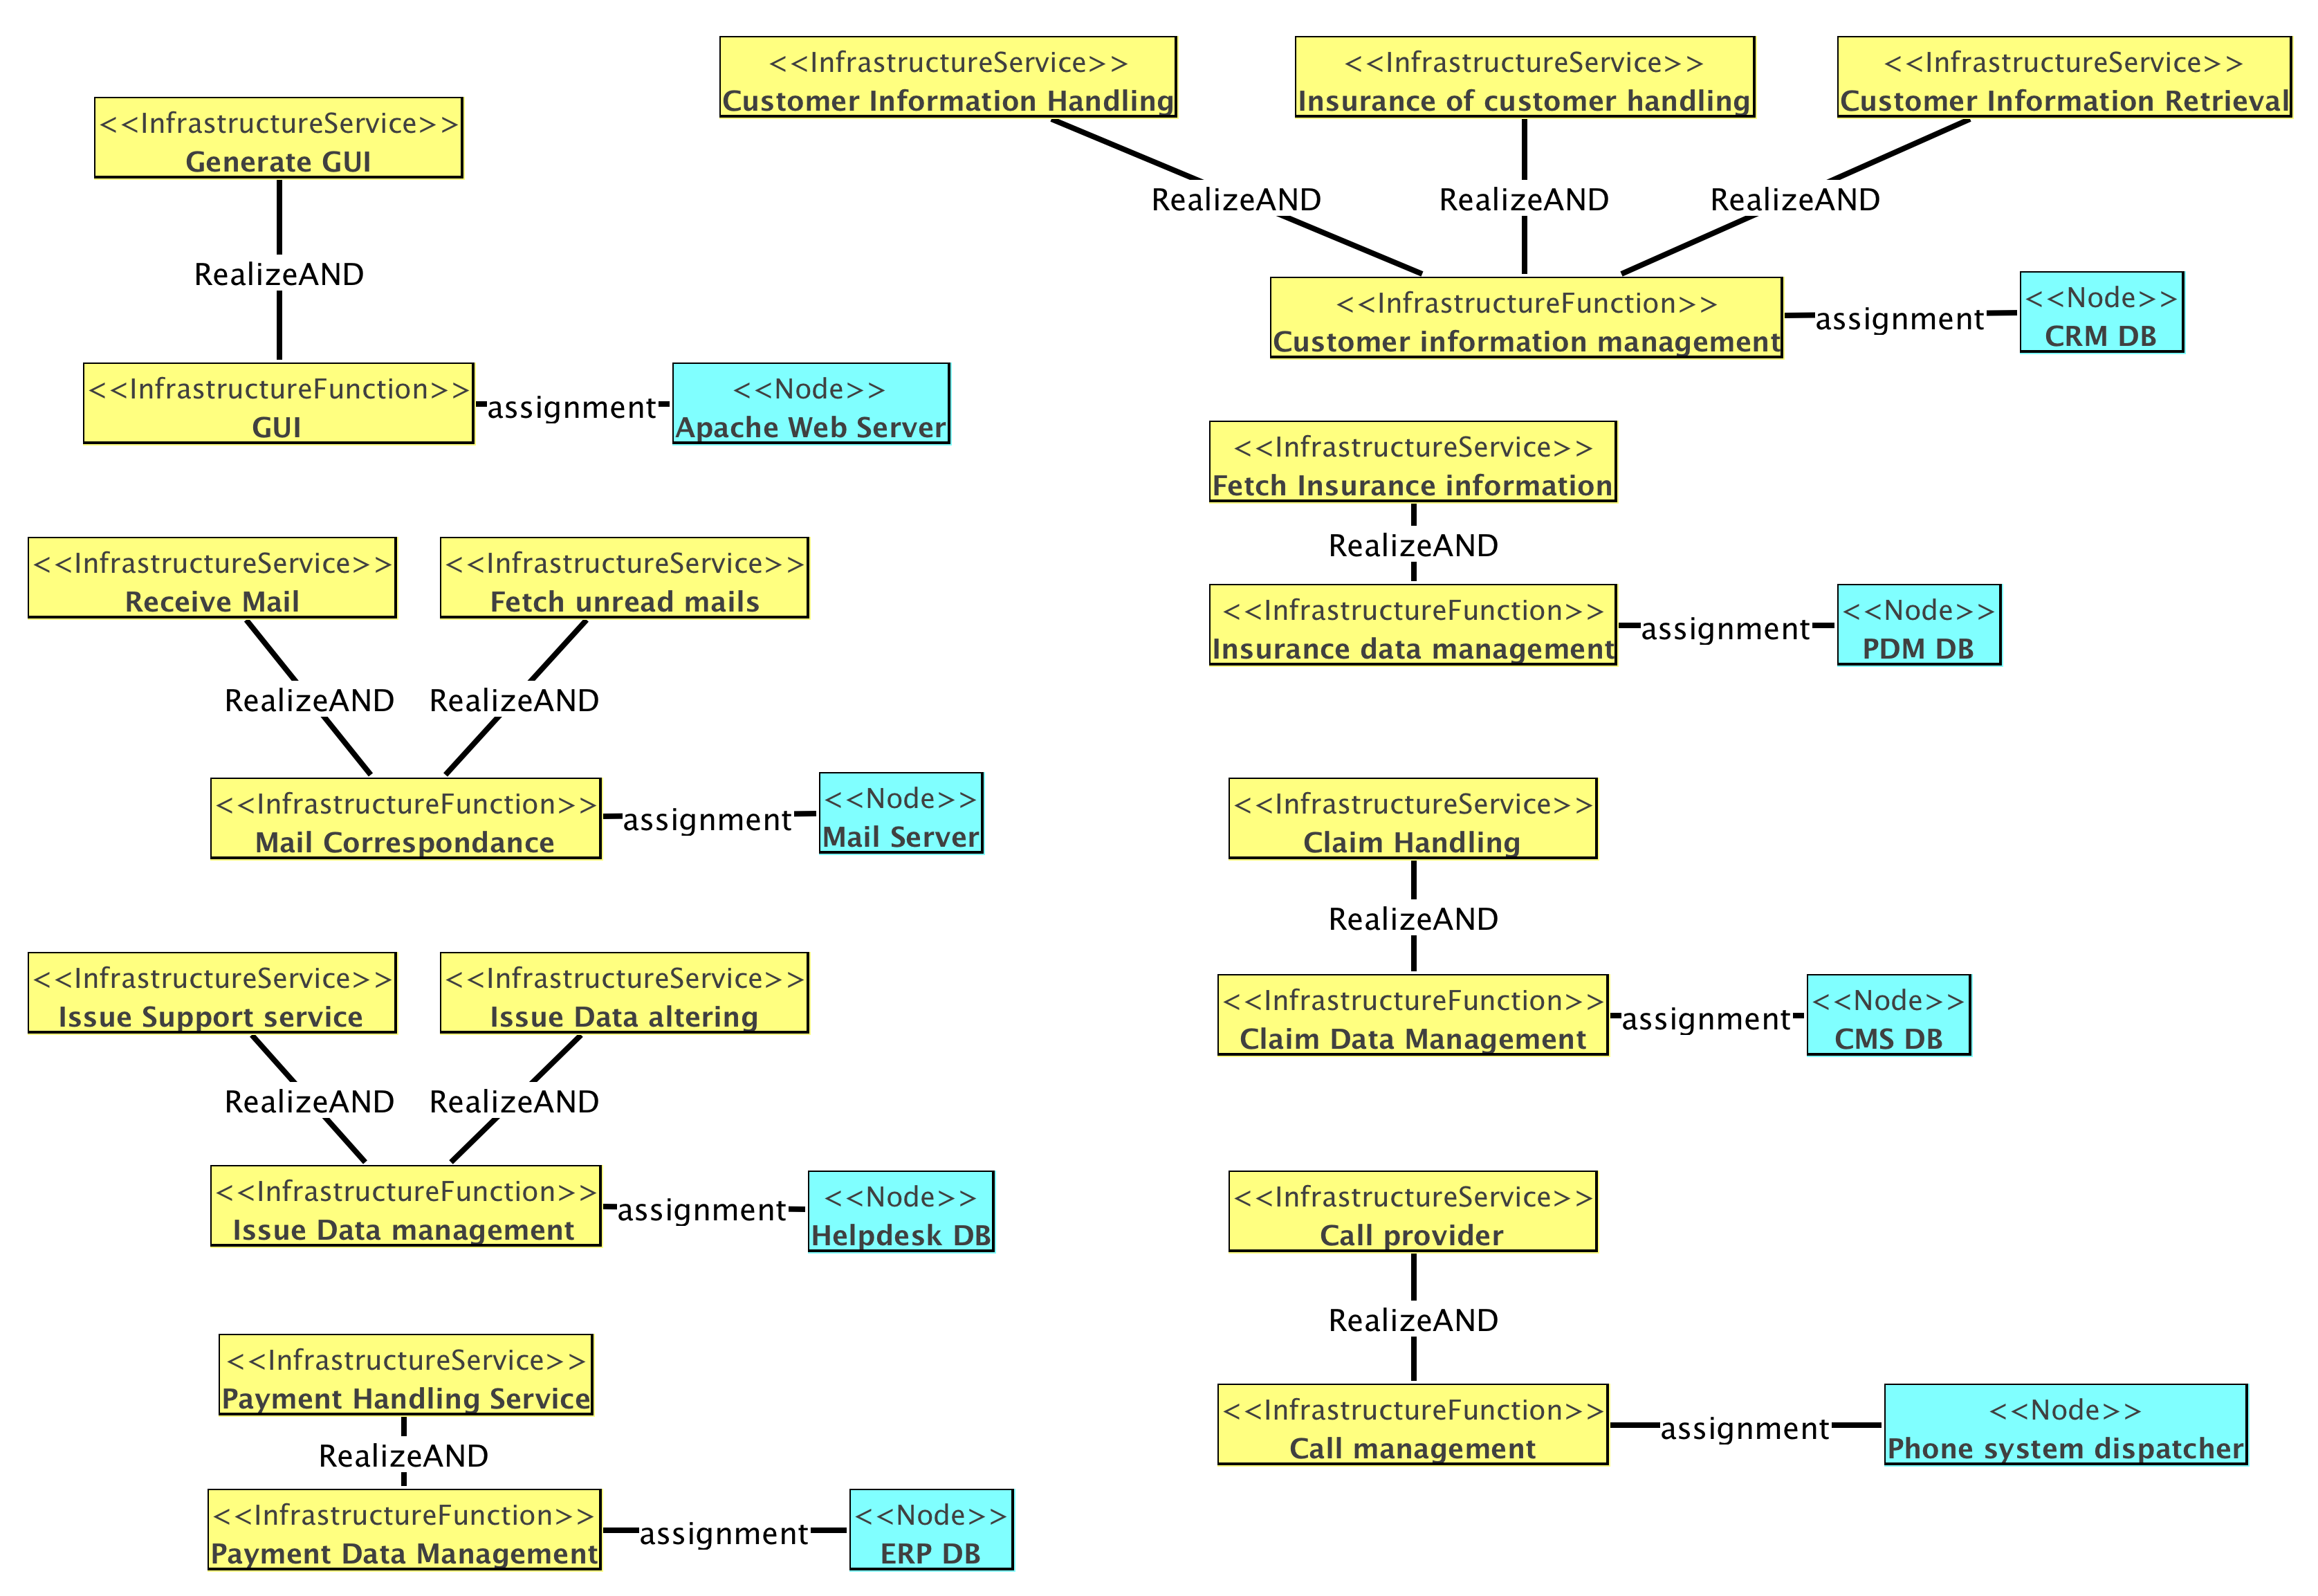
\includegraphics[scale = 0.12, angle=90]{images/map_infrastructure_tobe.png}}
		\caption{To-Be Infrastructre Architecture}
		\label{fig:map_information_to_be}
	\end{figure}
\end{center}
%\clearpage
 

\end{document}
